%%%%%%%%%%%%%%%%%%%%%%%%%%%%%%%%%%%%%%%%%%%%%%%%%%%%%%%%%%%%%%%%%%%%%%%%%%%%%%%%
% PHD DISSERTATION
%
%
% Michael Malick
% 2016-10-30
% v0.01
%
%%%%%%%%%%%%%%%%%%%%%%%%%%%%%%%%%%%%%%%%%%%%%%%%%%%%%%%%%%%%%%%%%%%%%%%%%%%%%%%%



% ----------------------------
% Pre-amble
% ----------------------------
% {{{

\documentclass[12pt]{report}
\usepackage{natbib}
\usepackage{pdflscape}
\usepackage{fancyhdr}
\usepackage{graphicx}
\usepackage{setspace}
\usepackage{pdfpages}
\usepackage{longtable}
\usepackage{threeparttable}  % provides table notes
\usepackage{threeparttablex} % enables table notes with long tables
\usepackage{fixltx2e} % provides \textsubscript
\usepackage[showframe=false, 
            includefoot, % ensure page numbers do not extend into margins
            includehead, % ensure page numbers do not extend into margins
            top=1.0in, 
            bottom=1.0in, 
            left=1.25in, 
            right=1.25in ]{geometry}
\usepackage{hyperref}
\hypersetup{pdfstartview=FitH,
            bookmarksopen=false,
            colorlinks,
            linkcolor=black,
            urlcolor=black,
            citecolor=black}
\usepackage{amstext}
\usepackage{amsmath}

%% Latin Modern Font
% \usepackage[T1]{fontenc}
% \usepackage{lmodern}
% \usepackage{cfr-lm} % latin-modern with old-style numbers

%% Free Bembo
% \usepackage[full]{textcomp}
% \usepackage[sups,osf]{fbb} % osf (or tosf) for text, not math
% \usepackage[scaled=.95]{cabin} % sans serif
% \usepackage[varqu,varl]{inconsolata} % sans serif typewriter
% \usepackage[libertine,bigdelims,vvarbb]{newtxmath} % bb from STIX
% \usepackage[cal=boondoxo]{mathalfa} % mathcal

%% Libertine font
%% http://get-software.net/fonts/newtx/doc/newtxdoc.pdf (pg. 7)
\usepackage[lining,semibold]{libertine} % a bit lighter than Times--no osf in math
\usepackage[T1]{fontenc} % best for Western European languages
\usepackage{textcomp} % required to get special symbols
\usepackage[varqu,varl]{inconsolata}% a typewriter font must be defined
\usepackage{amsthm}% must be loaded before newtxmath
\usepackage[libertine,cmintegrals,bigdelims,vvarbb]{newtxmath}
\usepackage[scr=rsfso]{mathalfa}
\usepackage{bm}% load after all math to give access to bold math
%% After loading math package, switch to osf in text.
\useosf % for osf in normal text

% Left justify the captions
\usepackage{caption}
\captionsetup{justification=justified,
              singlelinecheck=false}

\widowpenalty=1000
\clubpenalty=1000

% 1.5 line spacing
\onehalfspacing

% Line numbers
% \usepackage{lineno}
% \linenumbers

% change font of hyperlinks
\usepackage{url}
\urlstyle{rm}



\begin{document}
% \raggedright
\setlength{\parindent}{1cm}	
\bibpunct{(}{)}{;}{a}{}{;}


% }}}



% ----------------------------
% Includes
% ----------------------------
% \phantomsection is needed for 
% certain sections to have proper 
% links in the toc


% Title page
\pagenumbering{gobble}
% PHD THESIS TITLE PAGE
% Michael Malick
% 28 Aug 2015



\vspace*{3mm}
\begin{center}

\begin{spacing}{2.0}
{ \Large Ecological drivers of spatial and temporal variability in Pacific
salmon productivity}
\end{spacing}

\vspace{5mm}
by
\vspace{5mm}

\begin{doublespace}
Michael J. Malick  \\
M.Sc., University of Alaska Fairbanks, 2008 \\
B.Sc., Mansfield University, 2006 \\
\end{doublespace}

\vspace{10mm}
Thesis Submitted in Partial Fulfillment \\
of the Requirements for the Degree of \\

\vspace{5mm}
Doctor of Philosophy \\
\vspace{5mm}

in the \\
School of Resource and Environmental Management \\
Faculty of Environment \\

\vspace{10mm}
\copyright Michael J. Malick 2016 \\
SIMON FRASER UNIVERSITY \\
Summer 2016 \\

\vspace{15mm}
All rights reserved. \\
However, in accordance with the \emph{Copyright Act of Canada},
this work may be reproduced, without authorization, under the conditions for
``Fair Dealing''. Therefore, limited reproduction of this work for the purposes
of private study, research, criticism, review, and news reporting is likely to
be in accordance with the law, particularly if cited appropriately.


\end{center}




\clearpage
\pagenumbering{roman}
\setcounter{page}{2}

% Approval
\phantomsection
% PHD THESIS APPROVAL PAGE
% Michael Malick
% 28 Aug 2015 



\begin{center}
{ \Large \textbf{Approval} }
\end{center}
\addcontentsline{toc}{chapter}{Approval}

\vspace{4mm}

\hspace*{-1cm} \begin{tabular}{ l p{94mm} }
  \textbf{Name:} & Michael J. Malick \\
  \textbf{Degree:} & Doctor of Philosophy \\
  \textbf{Title of Thesis:} & Ecological drivers of spatial and temporal
  variability in Pacific salmon productivity \\

  & \\

  \textbf{Examining Committee:} & Dr. Andrew Cooper, Associate Professor \\
                                & Chair \\

    & \\ \cline{2-2}
    & Dr. Sean Cox, Senior Supervisor \\
    & Associate Professor \\
    & School of Resource and Environmental Management \\

    & \\ \cline{2-2}
    & Dr. Murray Rutherford, Supervisor \\
    & Associate Professor \\
    & School of Resource and Environmental Management \\

    & \\ \cline{2-2}
    & Dr. Franz Mueter, Supervisor \\
    & Associate Professor \\
    & School of Fisheries and Ocean Sciences\\
    & University of Alaska Fairbanks\\

    & \\ \cline{2-2}
    & Dr. Michael Bradford, Internal Examiner \\
    & Adjunct Professor \\
    & School of Resource and Environmental Management \\
    & Fisheries and Oceans Canada, Burnaby, B.C. \\

    & \\ \cline{2-2}
    & Dr. Louis Botsford, External Examiner \\
    & Professor \\
    & Department of Wildlife \\
    & University of Californis at Davis \\
    
    & \\
  \textbf{Date Approved:}  & \\  \cline{2-2}
\end{tabular}



\clearpage

% Partial copyright
\phantomsection
\addcontentsline{toc}{chapter}{Partial Copyright License}
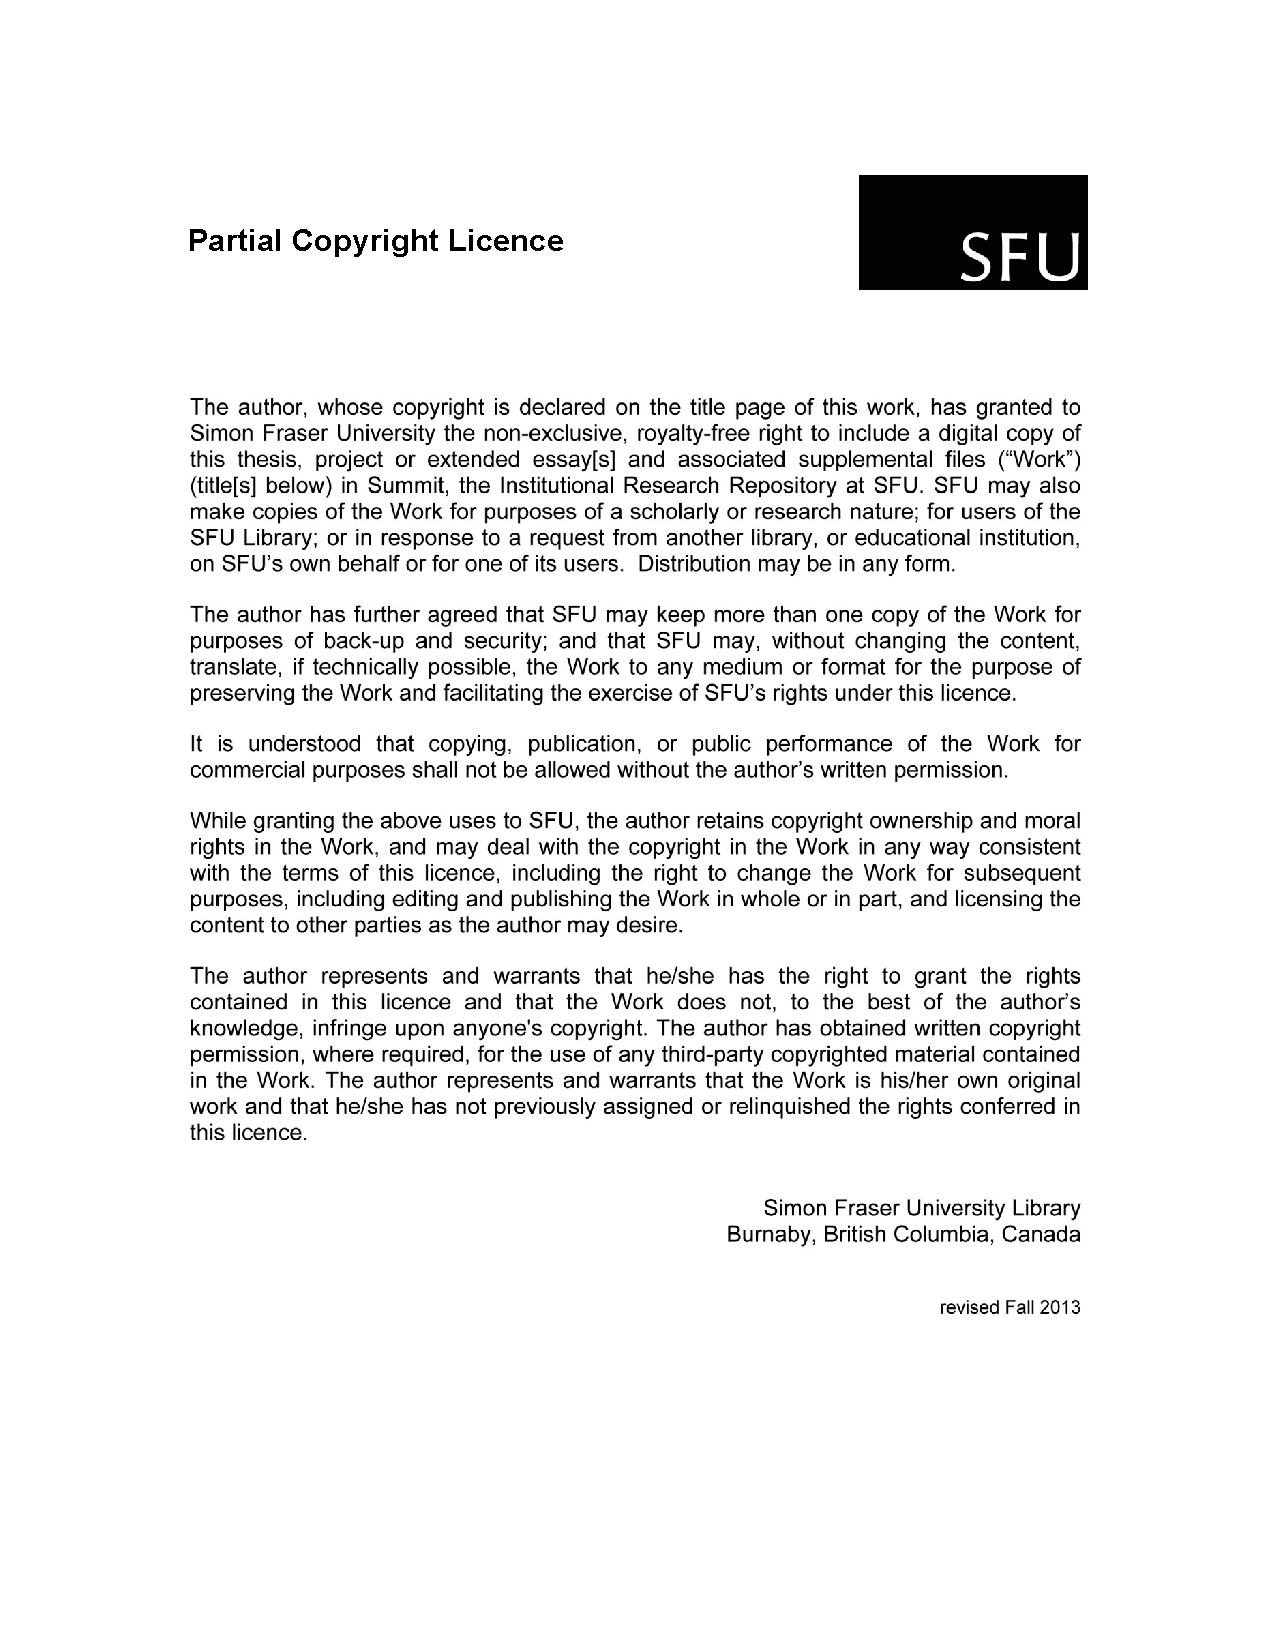
\includepdf[pagecommand={\thispagestyle{plain}}, pages={1}]
  {./1_frontmatter/partial-copyright.pdf}

% Abstract
%%%%%%%%%%%%%%%%%%%%%%%%%%%%%%%%%%%%%%%%%%%%%%%%%%%%%%%%%%%%%%%%%%%%%%%%%%%%%%%%
% PHD DISSERTATION ABSTRACT
%
%
% Michael Malick
% 10 Feb 2015  
%
%%%%%%%%%%%%%%%%%%%%%%%%%%%%%%%%%%%%%%%%%%%%%%%%%%%%%%%%%%%%%%%%%%%%%%%%%%%%%%%%


\chapter*{Abstract}
\addcontentsline{toc}{chapter}{Abstract}

Test of abstract page.

\clearpage

% Quote
%%%%%%%%%%%%%%%%%%%%%%%%%%%%%%%%%%%%%%%%%%%%%%%%%%%%%%%%%%%%%%%%%%%%%%%%%%%%%%%%
% PHD DISSERTATION ABSTRACT
%
%
% Michael Malick
% 10 Feb 2015  
%
%%%%%%%%%%%%%%%%%%%%%%%%%%%%%%%%%%%%%%%%%%%%%%%%%%%%%%%%%%%%%%%%%%%%%%%%%%%%%%%%



\vspace*{7cm}

\begin{flushright}

\emph{``Everything should be made as simple as possible, but not simpler''} \\
\emph{-- Albert Einstein}

\vspace*{2cm}

\emph{``If I have seen farther it is by standing on the shoulders of giants''} \\
\emph{-- Sir Isaac Newton}

\end{flushright}

\clearpage

% Acknowledgements
% PHD THESIS ACKNOWLEDGEMENTS
% Michael Malick
% 28 August 2015


\chapter*{Acknowledgements}
\addcontentsline{toc}{chapter}{Acknowledgements}

I sincerely thank my supervisors Randall Peterman and Sean Cox for their
guidance, advice, and encouragement. My success reflects their ability as
mentors and I am grateful for their inspiration and their willingness to allow
me the freedom to explore new paths. To Randall, you provided an exceptional
example of how to be a great scientist and I will always be grateful for the
opportunities you provided me at SFU. To Sean, you have been a source of
inspiration as a scientist and I am grateful for you welcoming me into your lab.

I have benefited greatly from the advice and  many insightful discussion with my
supervisory committee. I am grateful to Franz Mueter for being available to
discuss my research and taking the time to provide critical feedback on my
research.  I thank Murray Rutherford for his patience and guidance as I learned
the details of policy research and his clear and reliable insights to the policy
process.

I am grateful to the many people who participated as collaborators in my
research.  Thanks to Thomas Wainwright and Bill Peterson, who hosted me in
Newport, OR, and provided keen insights and guidance on the marine system off
the coast of Newport. I also thank Nathan Mantua and Todd Mitchell who hosted me
at the University of Washington and taught me the details of working with
satellite data sets.

To my fellow lab member in the fisheries group at SFU, thank you for providing
me a source of companionship and your willingness and enthusiasm to discuss
anything quantitative. I am grateful to my colleagues in the REM PhD program who
provided inspiration and a sounding board for me to discuss my research.

I thank the many biologists from the Washington Department of Fish and Wildlife,
Fisheries and Ocean Canada, the Alaska Department of Fish and Game, and the
Newport Research Station for collecting and providing me with the numerous data
sets analyzed here.  Without their efforts this research would not have been
possible.  

I am grateful for funding from the Canada Research Chairs Program provided to
Randall Peterman and to Simon Fraser University for the numerous scholarships
and fellowships that also supported my research.

It is beyond my abilities to thank my family for their encouragement during my
education. To my beautiful wife Erin, thank you for providing me a source of joy
and happiness everyday and your willingness to listen to me discuss the details
of my research. To my parents, brother, and extended family, thank you for your
unwavering support through all my years of education.  Mother and Dad, you have
always given me the freedom to pursue my interests and provided me with
unconditional encouragement, thank you.

My life has be greatly enriched by these individuals, and for that I am
grateful.



\clearpage

% TOC
\phantomsection
\addcontentsline{toc}{chapter}{Contents}
\tableofcontents
\clearpage

% List of tables
\phantomsection
\addcontentsline{toc}{chapter}{List of Tables}
\listoftables
\clearpage

% List of figures
\phantomsection
\addcontentsline{toc}{chapter}{List of Figures}
\listoffigures
\clearpage
\pagenumbering{arabic}
\setcounter{page}{1} 

%%%%%

% Fancy Headers
\fancyhf{}
\renewcommand{\headrulewidth}{0pt} % remove header rule
\pagestyle{fancy}
\lhead{\small \textit{\leftmark}}
\rhead{\small \thepage}
% \pagestyle{headings} % default latex header


% Introduction
\chapter{General Introduction}\label{general-introduction}

Test of section.

\clearpage

% Spring-bloom
\chapter{Linking phytoplankton phenology to salmon productivity along a
north-south gradient in the Northeast Pacific Ocean}


\section{Abstract}

We investigated spatial and temporal components of phytoplankton dynamics in the
Northeast Pacific Ocean to better understand the mechanisms linking biological
oceanographic conditions to productivity of 27 pink salmon (\emph{Oncorhynchus
gorbuscha}) stocks. Specifically, we used spatial covariance functions in
combination with multi-stock spawner-recruit analyses to model relationships
among satellite-derived chlorophyll-a concentrations, initiation date of the
spring phytoplankton bloom, and salmon productivity. For all variables, positive
spatial covariation was strongest at the regional scale (0-800 km) with no
covariation beyond 1500 km. Spring bloom timing was significantly correlated
with salmon productivity for both northern (Alaska) and southern (British
Columbia) populations, although the correlations were opposite in sign. An early
spring bloom was associated with higher productivity for northern populations
and lower productivity for southern populations. Furthermore, the spring bloom
initiation date was always a better predictor of salmon productivity than mean
chlorophyll-a concentration. Our results suggest that changes in spring bloom
timing resulting from natural climate variability or anthropogenic climate
change could potentially cause latitudinal shifts in salmon productivity.


\section{Introduction}

The dynamics of marine fish populations are often characterized by large
inter-annual and inter-decadal variability in abundances. For Pacific salmon
(\emph{Oncorhynchus} spp.), the first year of ocean residence is widely viewed
as a critical period that can strongly influence stock abundance
\citep{Peterman1985a, Parker1968a, Wertheimer2007a}. During this period,
climatic and oceanographic conditions are believed to strongly affect salmon
productivity (i.e., the number of adult recruits produced per spawner), yet the
ecological pathways connecting environmental variability to upper trophic levels
of marine food webs are not well understood \citep{Drinkwater2010a,
Ottersen2010a}. Evidence suggests that salmon mortality during the early marine
life stage is inversely related to body size, indicating that bottom-up forcing
mechanisms that affect prey resources may be an important part of these
ecological pathways \citep{McGurk1996a, Duffy2011, Farley2007b}.

Several bottom-up forcing mechanisms have been proposed to explain productivity
variation in marine fish stocks, including salmon \citep{Cushing1990a,
Gargett1997a}. For example, the ``optimal stability window'' hypothesis suggests
that changes in water column stability may be a critical component linking
changes in large-scale climate patterns and salmon productivity
\citep{Gargett1997a}. However, this hypothesis assumes a strong link between
phytoplankton dynamics (e.g., productivity or total biomass) and salmon
productivity, which is largely untested beyond a few local-scale studies
\citep{Mathews1989a, Chittenden2010a}.  Accounting for both spatial and temporal
variability of lower-trophic-level processes is a key challenge to testing the
optimal stability window hypothesis on large spatial scales.

In the coastal Northeast Pacific, seasonal biomass of phytoplankton follows a
well-known pattern defined primarily by the spring bloom \citep{Henson2007a,
Waite2013}, which is mainly driven by large-scale climate patterns combined with
regional and local-scale physical environmental conditions \citep{Sverdrup1953a,
Ware1991a, Polovina1995a, Henson2007a}. In the coastal Gulf of Alaska, the
spring bloom initiation date is strongly correlated with the onset of water
column stability, which is at least partially controlled by the strength of the
Aleutian Low Pressure system \citep{Henson2007a}. In that region, an earlier
spring bloom is also associated with a more intense bloom, suggesting that both
the phenology of the spring bloom and overall production during the bloom may be
important components of bottom-up forcing pathways. Indeed, features of the
spring bloom such as initiation date and total phytoplankton biomass are
correlated with yield and productivity of certain marine fish populations
\citep{Platt2003a, Ware2005a, Koeller2009}.

In this paper, we asked whether the spring bloom initiation date and average
chlorophyll-a (chl-a) concentrations (a surrogate for phytoplankton biomass) can
explain spatial and inter-annual variability in pink salmon (\emph{O.
gorbuscha}) productivity, which we estimated using spawner-recruit data for 27
stocks. Establishing a plausible mechanistic link between the spring
phytoplankton bloom and salmon production first requires evidence that the two
processes operate at similar spatial scales; that is, spatial covariation of
lower-trophic level processes should approximately match the spatial scale of
covariation observed in the salmon productivity data that they are being used to
explain \citep{Bjornstad1999a, Koenig1999a}. In the Northeast Pacific Ocean,
productivity of salmon stocks exhibit spatial synchrony at the scale of 100 to
1000 km \citep{Mueter2002b} with positive correlations being greatest at
distances less than 500 km \citep{Pyper2005a}. Therefore, we hypothesized that
features of the spring phytoplankton bloom operate at similar regional spatial
scales as salmon productivity.

We used spatial covariance analyses to determine the spatial extent of synchrony
in the timing of the spring phytoplankton bloom and mean chl-a concentrations
along the Northeast Pacific coast, as well as to determine the scale of spatial
averaging that should be used on data for these variables. We then used a
hierarchical, multi-stock statistical modeling approach to estimate
relationships between pink salmon productivity and inter-annual variability in
spring bloom initiation date, as well as mean chl-a concentration during spring
and late summer.  Compared to single-stock analyses, our multi-stock modeling
approach can help reduce uncertainty associated with the biological processes
that underpin the dynamics of salmon populations and reduce the chance of
finding spurious relationships by using different salmon stocks as replicates
within the analysis \citep{Myers1998c, Myers1999a}.


\section{Methods}

\subsection{Pink salmon data}

We estimated annual indices of productivity (in units of adult recruits per
spawner) for 27 wild pink salmon stocks from British Columbia (B.C.) and Alaska
(AK) using data on spawner abundance and total recruitment (catch plus
escapement). The 27 spawner-recruit data sets (Table 1) represent aggregations
of escapement and catch of adjacent salmon stocks. The aggregation helped ensure
that catches were attributed to the correct spawning stocks and was primarily
based on jurisdictional management units, although in some cases aggregation
occurred at a larger scale because of difficulty allocating catch into
individual management units (e.g., Prince William Sound). Hatchery returns were
excluded from all estimates of catch and escapement. Estimation methods for
spawner abundances varied among stocks, but in general, southern stocks (B.C.)
were estimated using expansions of foot surveys, while northern stocks (AK) were
estimated using expansions of aerial surveys (personal communication from data
sources listed in footnotes of Table 1). Annual recruitment varied widely among
stocks with long-term averages ranging from 0.12 million pink salmon for Chignik
Bay to 33.31 million for southern southeast Alaska (Table 1).

\subsection{Chlorophyll-a data}

We used satellite-derived chl-a concentration estimates (measured as mg
m\textsuperscript{-3}) from the Sea-viewing Wide Field-of-view Sensor (SeaWiFS)
and the Moderate Resolution Imaging Spectroradiometer (MODIS-Aqua) from the
Goddard Space Flight Center (\url{http://oceancolor.gsfc.nasa.gov}). Level-3
processed data were downloaded for 1998-2010 (but only 2003-2010 had complete
MODIS data) in their original 9 km\textsuperscript{2}, 1-day-resolution. We
converted the data to a 1$^{\circ}$x1$^{\circ}$ resolution and subsetted the
resulting grid to 46$^{\circ}$--61$^{\circ}$N and 167$^{\circ}$--125$^{\circ}$W,
including only grid cells adjacent to the coast (Fig.  1). We excluded grid
cells in the Bering Sea because all salmon stocks in our data set enter the
ocean in the Gulf of Alaska.

All analyses were performed using 8-day composite chl-a data because these had
less missing data across all years compared to 1-day and 5-day composites
(online Supplemental Fig. S1). In addition, the SeaWiFS data set had numerous
large gaps during the spring and summer for years 2008-2010, which made these
years of SeaWiFS data unsuitable for our study (online Supplemental Fig. S1). We
evaluated the feasibility of concatenating the SeaWiFS and MODIS data sets into
a single continuous data set that would provide an additional three years of
data (compared to using SeaWiFS data alone) by comparing the two data sets over
the first five overlapping years (2003-2007; online Supplemental data A). We
estimated correlations, root mean squared log\textsubscript{10} error (RMSE),
and log\textsubscript{10} bias to quantify differences between the two chl-a
data sets. The SeaWiFS and MODIS data sets were highly correlated (average of
0.87 across all grid cells). In addition, over all years and grid cells RMSE
(0.16) and log bias (0.012) (online Supplemental Fig. S2) were consistent with
other studies comparing SeaWiFS and MODIS data products over a similar study
region \citep{Waite2013}. Based on these minimal differences, we concatenated
the SeaWiFS (1998-2002) and MODIS (2003-2010) data sets without further
processing.

Inter-annual variability in phytoplankton standing stock and phytoplankton
phenology were quantified using mean monthly chl-a concentration and the
spring-bloom initiation date, respectively, which we derived from the 8-day
composite chl-a estimates for each grid cell (Fig. 1). We linearly interpolated
data points in chl-a time series for each grid cell between gaps less than 3
data points (4.1\% of all chl-a data points were interpolated). This procedure
was done prior to estimating annual spring bloom initiation date and mean chl-a
concentrations. We estimated the spring bloom initiation date as the first 8-day
period in a given year when the chl-a concentration was more than 5\% above the
median chl-a concentration of the entire multi-year data set for a particular
grid cell \citep{Siegel2002a, Henson2007a}. In addition, we
log\textsubscript{10}-transformed the chl-a averages to help normalize the chl-a
values.


\subsection{Spatial covariation analysis}

We constructed cross-correlation matrices to quantify spatial covariance
patterns for (1) pink salmon stock productivities, (2) spring-bloom initiation
dates, and (3) monthly mean chl-a concentrations. For salmon stocks, pairwise
correlation coefficients were computed between time series of productivity for
each of the 27 stocks. For the spring bloom initiation date, correlation
coefficients were computed between each pair of grid cells using time series of
the estimated annual spring bloom initiation date for years 1998-2010. For chl-a
concentration, we calculated correlations across grid cells using time series of
the monthly mean chl-a concentration. To account for potential changes in
spatial patterns across seasons, we calculated correlations for chl-a
concentration for each month (February-October) separately.

We estimated annual salmon productivity using residuals from a Ricker
spawner-recruit model, which removed potential within-stock
density-dependent effects \citep{Pyper2001a, Mueter2002a, Ricker1954a}.
The Ricker model for each stock was of the form,

\begin{equation}
log_e(R_{i,t} / S_{i,t}) = \alpha_i + \beta_i S_{i,t} + \epsilon_{i,t},
\label{eq:bloom:1}
\end{equation}

\noindent
where \(R_{i,t}\) is total pink salmon recruits for the \(i^{th}\) stock in
brood year \(t\), \(S_{i,t}\) is the spawning stock two years earlier,
\(\alpha_i\) is the maximum log\textsubscript{e} recruits-per-spawner,
\(\beta_i\) is the coefficient of density-dependence, and \(\epsilon_{i,t}\) is
the residual.

We fit the Ricker models (eq. \ref{eq:bloom:1}) to two partitions of the data -- one
including all available brood years and the second including only brood years
1997-2009 (Table 1). The latter partition corresponds to the years available for
the bloom initiation date and chl-a variables. Because juvenile pink salmon
enter the ocean the year following spawning (i.e., brood year + 1), we offset
the phytoplankton variables one year to correspond with the ocean entry year for
pink salmon (e.g., 2006 brood year was lined up with 2007 phytoplankton
variables).

To test whether spatial covariation was present in each of the variables, we
first performed Mantel tests using matrices of the cross-correlations and a
matrix of great-circle distance (computed using the haversine formula) between
all pairs of grid cells or stocks \citep{Legendre1998a, Koenig1999a}.
Statistical significance of Mantel statistics were determined using
randomization tests with 1 000 permutations. We then determined the spatial
scale of covariation for each significant Mantel test by fitting a smooth
non-parametric covariance function \citep{Bjornstad2001a} between the
correlation coefficients for a given variable and the distance separating
correlated grid cells or ocean-entry points of salmon stocks. Confidence
intervals (CI) for each covariance function were computed by bootstrapping the
estimation procedure 1 000 times.

Covariance functions were summarized using two distance metrics: (1) the
y-intercept of the covariance function, which provides an estimate of the
correlation at zero distance (CZD), and (2) 50\% correlation scale (D50). The
CZD was estimated by extrapolating the fitted covariance function to zero
distance to find the y-axis intercept. The D50 was estimated as the distance at
which the covariance function falls to 50\% of its observed maximum value, which
provides a useful metric of how much the correlation declines with increasing
distance between salmon stocks or grid cells \citep{Mueter2002b}.

\subsection{Salmon productivity models}

We used a combination of single-stock linear models and multi-stock linear
mixed-effects models to investigate relationships among temporal averages of
mean chl-a concentrations (spring and late summer), spring bloom initiation
date, and pink salmon productivity. The single-stock model analysis had two
purposes. First, we used the values of fitted coefficients for different stocks
to inform construction of the multi-stock models and to help evaluate the
multi-stock model assumptions. Second, we used the single-stock analysis along
with intervention analyses to break up the data sets spatially to provide the
best fits of the multi-stock models. For both single-stock and multi-stock
models, only pink salmon brood years 1997-2009 were used.

The bloom initiation date and both chl-a covariates included in the models
represented spatial and temporal (for chl-a) averages of conditions experienced
by juvenile pink salmon during their early marine life phase. The bloom
initiation covariate was calculated for each salmon stock as the average of grid
cell specific anomalies (i.e., a grid cell's value minus the long term mean for
that grid cell) over all grid cells whose centers were within 250 km of the
stock's ocean entry point. For chl-a, we calculated April-May averages to
capture variability in phytoplankton biomass during the spring bloom and
July-September averages to index chl-a variability during the late summer, which
is believed to be a critical period for juvenile salmon survival
\citep{Beamish2001a, Moss2005a}. For both time periods, we first averaged chl-a
values over the specified months for each grid cell and then averaged over all
grid cells within 250 km of the stock's ocean entry point.

\subsubsection{Single-stock models}

The single-stock Ricker models took the form \citep{Adkison1996b},

\begin{equation}
log_e(R_{i,t} / S_{i,t}) = \alpha_i + \beta_i S_{i,t} + \gamma_i
X_{i,t+1} + \epsilon_{i,t}, \label{eq:bloom:2}
\end{equation}

\noindent
where \(S_{i,t}\) is spawner abundance of pink salmon in brood year \(t\) for
the \(i^{th}\) stock, \(R_{i,t}\) is the total recruitment resulting from
\(S_{i,t}\), \(\alpha_i\) indicates stock productivity at low spawner
abundances, \(\beta_i\) indicates the magnitude of density-dependence,
\(X_{i,t+1}\) is a stock-specific measure of either the spring bloom initiation
date or mean chl-a concentration (the latter for either the spring or late
summer), \(\gamma_i\) is the coefficient for either the stock-specific bloom
initiation date or mean chl-a, and \(\epsilon_{i,t} \sim N(0, \sigma^2)\) is an
independent and identically distributed residual term.

Environmental variables such as sea surface temperature could have opposite
effects on northern and southern pink salmon stocks \citep{Mueter2002a,
Su2004a}; therefore we used an intervention model with two means
\citep{Chatfield2004, Mueter2002a} to test for differences in the effect of the
bloom initiation date and chl-a concentration between northern and southern
stocks \citep{Chatfield2004, Mueter2002a}. The intervention models were fit to
either the estimated chl-a or spring bloom coefficients from the single-stock
models (i.e., \(\gamma\) in eq. \ref{eq:bloom:2}) where the coefficients were
arranged south to north based on ocean entry locations (i.e., by stock number in
Table 1).


\subsubsection{Multi-stock models}

We used hierarchical, multi-stock models to estimate both regional and
stock-specific effects of spring and late summer chl-a and the bloom initiation
date on pink salmon productivity, while also accounting for heterogeneity in
density-dependence among stocks. The multi-stock mixed effects Ricker models
took the form \citep{Myers1999a, Mueter2002a},

\begin{equation}
log_e(R_{i,t}/S_{i,t}) = \alpha + a_i - \beta_iS_{i,t} + 
X_{i,t+1} (\gamma_{X} + g_{i}) + \epsilon_{i,t}, \label{eq:bloom:3}
\end{equation}

\noindent
where the fixed intercept \(\alpha\) is the overall mean productivity common to
all stocks and \(a_i\) is the stock-specific deviation from that mean,
\(\beta_i\) is the fixed stock-specific density-dependent effect, \(X_{i,t+1}\)
represents either the spring bloom initiation date or mean chl-a concentration
(either spring or late summer average), \(\gamma_X\) is the overall mean effect
of either the spring bloom initiation date or mean chl-a concentration, \(g_i\)
is the stock-specific deviation from that overall mean for a particular chl-a
variable, and \(\epsilon_{i,t}\) is an independent and identically distributed
residual term (i.e., \(\epsilon_{i,t} \sim N(0,\sigma^2)\)).  The stock-specific
random effects \(a_i\) and \(g_i\) are assumed to follow a joint normal
distribution with means zero, variances \(\sigma^2_a\) and \(\sigma^2_g\), and
covariance \(\sigma^2_{ag}\).

Because the chl-a and bloom initiation variables were moderately correlated
(average correlations between stock-specific phytoplankton time series ranged
from -0.50 to 0.20), the multi-stock models were fit separately for the bloom
initiation date and both chl-a metrics. For the bloom initiation date and spring
chl-a variables, we also fit multi-stock models separately for a southern stock
group (stocks 1-9 in Table 1) and a northern stock group (stocks 10-27 in Table
1), because the single-stock analysis and intervention models suggested
consistent differences in the effects of these variables between northern and
southern stock groupings (see Results). For the late summer chl-a variable, we
fit a single model using all stocks because the intervention models did not
indicate a significant break between northern and southern stock groupings.

In addition to the full models (eq. \ref{eq:bloom:3}) for both chl-a variables and the bloom
initiation date, we investigated two simpler nested models, (1) eq. \ref{eq:bloom:3} but
without the random chl-a or bloom effect (i.e., \(g_{i}\)), and (2) eq. \ref{eq:bloom:3} but
without either the random or fixed chl-a or bloom effect (i.e., \(g_{i}\) and
\(\gamma_{X}\), which was the null model).  Random effect significance was
determined using likelihood ratio (L) tests among the nested models, whereas
fixed effect significance was tested using F-tests \citep{Pinheiro2000a}. All
reported parameters were estimated using restricted maximum likelihood methods;
however, for model comparisons, parameters were estimated using maximum
likelihood methods to reduce bias \citep{Pinheiro2000a}.

To compare the relative importance of the bloom initiation date and both chl-a
variables, we also calculated the small-sample Akaike Information Criterion
(AIC\textsubscript{C}) for all models \citep{Hurvich1989a, Burnham2002a}. For
the models that included late summer chl-a, which were fit using all 27 salmon
stocks, we calculated a single set of AIC\textsubscript{C} values (one for each
nested model).  For the models that included either the bloom initiation date or
spring chl-a variables, we calculated two sets of AIC\textsubscript{C} values.
First, to compare the relative importance of both variables within the northern
and southern areas, we calculated AIC\textsubscript{C} values for each model fit
to the northern and southern stock groups separately.  Second, to compare
variable importance with the late summer chl-a variable, we calculated an
AIC\textsubscript{C} value for the combined northern and southern models.
Because northern and southern models for the bloom initiation date and spring
chl-a variables were fit using identical salmon data as the late summer chl-a
models, we calculated a combined northern and southern AIC\textsubscript{C}
value for each variable by summing the log-likelihoods and the number of model
parameters. To more easily compare models, we also calculated the
\(\Delta\)AIC\textsubscript{C}, i.e., the difference between each individual
model's AIC\textsubscript{C} value and the minimum AIC\textsubscript{C} value
among models. Models within three AIC\textsubscript{C} units of the model with
the lowest AIC\textsubscript{C} value are considered equally plausible
\citep{Burnham2002a}.


\subsection{Sensitivity analysis}

We checked the sensitivity of our results to four assumptions. First, we
estimated sensitivity of the spatial analysis results to an alternative
Beverton-Holt stock-recruitment model \citep{Beverton1957a}
(log\textsubscript{e}(R/S) = log\textsubscript{e}(a) - log\textsubscript{e}(1 +
bS) + \(\epsilon\)). Second, we checked the sensitivity to the interpolation
procedure used on the chl-a time series by re-running each analysis using spring
bloom and chl-a values that did not include interpolated data points. Third, we
tested our assumption that the error terms of the multi-stock models were
temporally independent by refitting the models with first-order autocorrelated
errors (i.e., \(\epsilon_{i,t} = \phi\epsilon_{i,t-1} + \upsilon_t\), where
\(\upsilon_t \sim N(0, \sigma^2)\)) and using likelihood ratio tests to
determine the significance. Fourth, because our spawner-recruit data sets
include variability associated with both freshwater and marine life phases, we
checked the sensitivity of our results to the source of pink salmon data by
comparing each chl-a metric to pink salmon marine survival rates for three
Alaska hatchery stocks (Armin F.Koernig, Kitoi Bay, and Port Armstrong) using
Pearson correlation coefficients (see online Supplemental data B for details of
the analysis).


\section{Results}

\subsection{Spatial analysis}

Both sets of pink salmon residuals, monthly mean chl-a, and bloom initiation
date all showed significant spatial covariation (P \textless{} 0.01 for all
Mantel tests). For both sets of pink salmon residuals (all brood years and
recent, satellite-covered years), the nonparametric covariance functions
indicated declining positive covariation with increasing distance between ocean
entry points of juvenile salmon, up to approximately 800 to 1000 km where the
functions approached zero correlation (Fig. 2a and b). The estimated D50 was
slightly larger for productivity indices fitted using all available brood years
(D50 = 305 km; 95\% CI = 218-488 km) than for indices fitted using only brood
years 1997-2009 (D50 = 261 km; 95\% CI = 148-628 km), although there was
considerable overlap in confidence intervals (Figs. 2 and 3a). Correlations at
zero distance (i.e., the y-intercept of the covariance function) for both sets
of productivity indices were considerably less than one (CZD = 0.51; 95\% CI =
0.41-0.62 and CZD = 0.49; 95\% CI = 0.28-0.69 for all brood years and 1997-2009
respectively; Fig. 3b). Although the nonparametric covariance function for bloom
initiation date had a slightly larger D50 (D50 = 367 km; 95\% CI = 235-776 km)
than the two salmon productivity indices, there was considerable overlap in
confidence intervals with both productivity indices (Fig. 3a). Correlation at
zero distance for the bloom initiation date was also considerably less than one
(CZD = 0.44; 95\% CI = 0.33-0.55; Fig. 3b).

For monthly mean chl-a concentrations, covariation decayed steeply with
increasing distance over spatial scales of 0-500 km for all months (Fig.  4).
The D50 was highest (\textasciitilde{}380 to 430 km) during the winter and
spring (February-May) and declined to about 250 km during summer and fall
(June-October), which was similar to the estimated D50 for salmon productivity
(Fig. 5). In addition, confidence intervals for the chl-a D50 for all months
overlapped the confidence intervals for salmon productivity D50s (Fig. 5). The
CZD for chl-a concentrations ranged from 0.56 in June to 0.76 in April, which
was slightly higher than the estimated CZD for the bloom initiation date and
salmon productivity.


\subsection{Single-stock models}

The single-stock Ricker models indicated that pink salmon productivity was
related to the spring bloom initiation date either positively (15 stocks) or
negatively (12 stocks) (Fig. 6a). The distribution of model coefficients (i.e.,
\(\gamma\) in eq. \ref{eq:bloom:2}) ranged from -0.55 to 0.25 and was asymmetric
about zero with the majority of values between -0.2 and 0.25 (Fig. 6d).
Productivity of all 9 pink salmon stocks south of northern southeast Alaska
(i.e., stocks 1-9 in Table 1) was positively related to the spring bloom
initiation date, whereas productivity of northern stocks was mostly negatively
related (12 of 18 stocks; Fig.  6a). The intervention model indicated a
significant break (P \textless{} 0.05) in the sign of these relationships near
55.7$^{\circ}$N, which was between the southern southeast Alaska stock (stock 9)
and the northern southeast Alaska outside stock (stock 10; Fig. 1).

Pink salmon productivity was also both positively (14 stocks) and negatively (13
stocks) related to spring chl-a concentrations (Fig. 6b) with the coefficients
ranging from -3.4 to 6.0 (Fig. 6e). Like the bloom initiation date, the
intervention model indicated a significant break (P \textless{} 0.05) between
stocks 9 and 10 for the spring chl-a coefficients (Fig. 6b). Productivity for
all but two stocks in the southern group had a negative relationship with spring
chl-a concentrations, whereas the northern group had a mix of positive and
negative relationships.

For the late summer chl-a variable, productivity was consistently negatively
related to chl-a, with only 4 of the 27 stocks having a positive relationship
(Fig. 6c). The coefficients were approximately normally distributed with the
magnitudes ranging from -8.6 to 3.2 with a median value of -1.9 (Fig. 6f). In
contrast to the other two phytoplankton variables, the intervention model did
not indicate a significant break in the sign of the coefficients between
northern and southern stocks (Fig. 6c).

The productivity parameters (\(\alpha\)) for the bloom initiation date and both
chl-a models were approximately normally distributed (a requirement for the
multi-stock models), but the distribution of the density-dependent coefficients
(\(\beta\)) had a long left tail (online Supplemental Fig. S3).

\subsection{Multi-stock models}

Over all pink salmon stocks we considered, productivity was significantly
related to spring bloom initiation date (northern and southern models), spring
chl-a concentrations (southern model only), and late summer chl-a (\(\gamma\) in
Table 2), although stock-specific differences were not significant in any
models. For the bloom initiation date, regional effects were opposite in sign
for the northern and southern stock groups (\(\gamma\) in rows 2 and 5 in Table
2, Fig. 6a), suggesting that salmon productivity for the southern stock group is
higher than average when the bloom is later (positive coefficient), whereas
productivity is higher than average for the northern stock group when the bloom
is early (negative coefficient). This result contrasts with those for spring
(southern model only) and late summer chl-a, where the regional effect was
negative, implying reduced salmon productivity when chl-a concentrations are
higher (\(\gamma\) in rows 6 and 10 in Table 2). Furthermore, the spring bloom
initiation date was a better predictor of salmon productivity than mean chl-a
concentration for all subsets of data (i.e., northern stock group, southern
stock group, and all stocks) (AIC\textsubscript{C} values in Table 2).

Estimates of the regional effect of the spring bloom initiation date on salmon
productivity were significantly different than zero for both northern and
southern multi-stock models (\(\gamma\) in rows 2 and 5 in Table 2), but the
models were not significantly different than the full model (eq. \ref{eq:bloom:3}), which
included both the regional and stock-specific effects (L = 0.03, P
\textgreater{} 0.1). The estimated region-wide effect of spring chl-a
concentrations on salmon productivity of southern stocks and late summer chl-a
on productivity of all stocks were significantly different from zero (\(\gamma\)
in rows 6 and 10 in Table 2). However, for both models and chl-a variables,
there was no evidence of stock-specific effects based on likelihood ratio tests
comparing the full models to a model without the random chl-a effects (L =
0.001, P \textgreater{} 0.1 for both spring and late summer chl-a). In addition,
for the northern stock group there was no support for either a regional or
stock-specific effect of spring chl-a (row 3 in Table 2; L = 0.001, P
\textgreater{} 0.1).

In both the northern and southern areas, the bloom initiation date had a
stronger effect on pink salmon productivity than spring chl-a concentrations as
shown by the \(\Delta\)AIC\textsubscript{C} of 5.4 between the best fit models
for chl-a and the bloom initiation for the northern stock group and 12.5 for the
southern stock group (Table 2).  The bloom initiation date also had the highest
relative importance (\(\Delta\)AIC\textsubscript{C} = 0) when the northern and
southern models were combined with an AIC\textsubscript{C} value considerable
less than late summer chl-a, spring chl-a, and the null model (rows 7-10 in
Table 2). Between the two chl-a variables, the late summer chl-a average had a
higher relative importance (i.e., lower AIC\textsubscript{C} value) than the
average spring chl-a concentration as indicated by the 10 unit difference
between AIC\textsubscript{C} values (rows 9 and 10 in Table 2).

\subsection{Sensitivity analysis}

Our estimates of the spatial covariation in pink salmon productivity were not
sensitive to the form of stock-recruit model because residuals from the Ricker
and Beverton-Holt models were highly correlated (average correlation across
stocks = 0.97). The D50 and CZD values were nearly identical between models fit
using the Ricker and Beverton-Holt residuals. Similarly, the spatial analyses
were not sensitive to the interpolation of data points in the chl-a time series.
Difference between D50 values for the interpolated and non-interpolated spring
bloom series was 10 km, with almost complete overlap of the confidence
intervals. In addition, changes in D50 for monthly chl-a without interpolation
values ranged from 0 km to 10 km across months with almost complete overlap of
the confidence intervals. Coefficients of the multi-stock Ricker model were also
insensitive to the interpolation of missing data.

The results from the multi-stock models were not sensitive to our initial
assumption of uncorrelated errors. Specifically, the single-stock models did not
indicate strongly autocorrelated errors, and adding an autocorrelated error term
to the best-fit multi-stock models did not significantly improve the fits for
any of the models, which is consistent with other research on pink salmon
productivity \citep{Pyper2001a}. In addition, comparisons between the three
chl-a metrics and hatchery marine survival rates broadly agreed with the results
of the multi-stock models (online Supplemental data B and Fig.  S4).

\section{Discussion}

We investigated two indices of phytoplankton dynamics, spring bloom initiation
date and mean chl-a concentration, to better understand the potential mechanisms
linking biological oceanographic conditions to Pacific salmon productivity. Our
results indicated that (1) spatial covariation patterns for the spring bloom
initiation date, average chl-a concentration, and pink salmon productivity were
similar, with strongest positive covariation at the regional scale (0-800 km),
(2) there were opposing effects of the spring bloom initiation date on northern
and southern pink salmon stock productivity with an early bloom initiation date
being associated with higher northern stock productivity and a late bloom being
associated with higher southern stock productivity, (3) phytoplankton biomass
during the late summer (July-September) was more strongly associated with salmon
productivity than phytoplankton biomass during the spring (April-May), and (4)
the spring bloom initiation date was a better predictor of salmon productivity
than mean chl-a concentration for both southern and northern stocks.

Spatial synchrony for all three variables was strongest at regional spatial
scales and declined rapidly with increasing distance. For the bloom initiation
date and chl-a concentration, this suggests that physical processes operating on
relatively small spatial scales (e.g., summer sea surface temperature and sea
surface salinity) drives the spatial variability, rather than larger-scale
atmospheric processes such as the Pacific Decadal Oscillation
\citep{Mueter2002b}. For pink salmon productivity, our results suggest that both
phytoplankton biomass and the bloom initiation date could be factors driving the
regional-scale covariation. Furthermore, the match in spatial synchrony between
both phytoplankton variables and salmon productivity supports the inclusion of
these variables in the single-stock and multi-stock models and also lends
support for the observed correlations between pink salmon productivity and both
phytoplankton variables.

Spatial correlation of all three variables was less than one at zero distance,
indicating the presence of a ``nugget effect'', which represents variability due
to sampling error or spatial dependence at smaller scales than those sampled
\citep{Cressie1993}. For pink salmon productivity, this could be caused by
errors enumerating spawner abundances. For chl-a and the bloom initiation date,
the nugget effect may be caused by measurement errors in the chl-a estimates and
spatial averaging, or from the presence of small-scale oceanographic features
such as tidal mixing or river plumes that can lead to large changes in the bloom
initiation date and chl-a concentrations over short distances (\textless{} 100
km) \citep{Henson2007a}. The latter process could reduce the explanatory power
of both phytoplankton variables for salmon productivity because the
phytoplankton variables may not index conditions that salmon actually experience
at small spatial scales.

There was a marked reduction in the D50 for monthly chl-a concentrations between
May and June. The winter and spring period (February-May) included months with
both the highest annual chl-a concentrations (April and May) and the lowest
(February and March), whereas the chl-a concentrations during June-October were
relatively constant (online Supplemental Fig. S5). These periods correspond to
times before the spring bloom (February and March), during it (April and May),
and after it (June-October). Our results also showed that coherence in chl-a
concentrations following the spring bloom is smaller than prior to and during
the bloom, which may result from different mechanisms underlying the spatial
synchrony at different periods. For example, spatial synchrony before and during
the bloom may be primarily driven by regional-scale physical oceanographic
conditions such as sea surface temperature or sea surface salinity
\citep{Henson2007a}. In contrast, the period after the bloom also tends to
correspond to the period of peak zooplankton abundances in the Northeast
Pacific, indicating that chl-a concentrations after the bloom may be more
influenced by top-down grazing pressure, as suggested by others
\citep{Chittenden2010a, Bornhold2000, Mackas2012}.

A plausible explanation for the opposite effects of the bloom initiation date on
productivity of northern and southern stocks is that the spring bloom initiation
date is a surrogate for other processes that have direct effects on salmon
productivity such as predator abundances or zooplankton distributions. The
dividing line between the northern and southern stocks occurred in southern
southeast Alaska, which falls in the transition zone between the northern
downwelling domain and southern upwelling domain \citep{Ware1989a}. In the
northern region, the spring bloom initiation date has been shown to be closely
linked to the timing of water column stability, which is primarily determined by
freshwater runoff in the spring \citep{Weingartner2005a, Henson2007a}. Moreover,
both stability and the bloom initiation date in the northern domain tend to
occur earlier in warmer, wetter years that are associated with a more intense
Aleutian Low, higher zooplankton biomass, and increased salmon productivity
\citep{Brodeur1992a, Mueter2002a}. In the southern domain, an earlier spring
bloom is also associated with increased water column stability, however,
stability in this region is primarily driven by increased thermal warming and
reduced upwelling-favorable winds, both of which are also associated with a
stronger Aleutian Low \citep{Polovina1995a, Henson2007a}. In contrast to the
northern domain, these conditions in the south for an early bloom initiation
have been shown to be associated with increased predator abundances, reduced
zooplankton biomass, and decreased salmon productivity \citep{Ware1995a,
Mackas2001a, Mueter2002a}.

The optimal stability window hypothesis \citep{Cury1989a, Gargett1997a} provides
another possible explanation for the opposite effects of the bloom initiation
date on productivity of northern and southern stocks.  This bottom-up forcing
mechanism posits that synchronous changes in water column stability in northern
and southern areas, which are driven by strength of cyclonic circulation in the
Gulf of Alaska \citep{Gargett1997a}, can lead to out-of-phase salmon survival
rates between the two areas. However, the degree to which our results support
the optimal stability window hypothesis depends on the extent to which (1) water
column stability and the spring bloom initiation date are linked, (2) water
column stability has opposite effects on primary production in northern and
southern regions, and (3) there is a strong positive relationship between
phytoplankton biomass and salmon productivity. Although the first two
relationships are beyond the scope of this research, our results indicate that
there is only a weak relationship between phytoplankton biomass during the
spring and salmon productivity and a stronger but negative relationship between
phytoplankton biomass during the late summer and salmon productivity.

The latitudinal shift in the effect of the spring bloom initiation date on
northern and southern stock productivity corresponds with previous studies that
showed opposite effects of sea surface temperature on the productivity of
northern and southern pink salmon, chum salmon (\emph{O.  keta}), and sockeye
salmon (\emph{O. nerka}) stocks \citep{Mueter2002a, Su2004a}. In particular,
\citet{Mueter2002a} and \citet{Su2004a} indicated that warm sea surface
temperatures were associated with higher pink salmon productivity for northern
stocks and lower productivity for southern stocks with the north/south break
occurring near the southern end of Southeast Alaska
(\textasciitilde{}54$^{\circ}$N), which closely matches the break point we
identified for the spring bloom initiation date
(\textasciitilde{}56$^{\circ}$N).  This consistency in the latitude of the
north/south break point across studies of different environmental variables
further supports the idea that the opposite effects are driven by differences in
ocean conditions between the northern and southern domains.

It is not clear why a lower late summer chl-a concentration would be associated
with greater salmon productivity, but a possible explanation relates to top-down
grazing pressure. Our chl-a variable represents variability in the phytoplankton
standing stock, which can be influenced by both phytoplankton productivity and
top-down grazing pressure.  Zooplankton grazers in the Northeast Pacific at
least partially control the standing stock of phytoplankton \citep{Strom2001,
Frost1987} and, in turn, are an important food source for juvenile pink salmon
\citep{Boldt2003a, Armstrong2005a, Beauchamp2007a}. If pink salmon do not
significantly control zooplankton abundance, then lower phytoplankton biomass
could represent higher zooplankton abundances available to support higher growth
and survival of pink salmon. This hypothesis is supported by observations in the
Strait of Georgia, British Columbia indicating that peak zooplankton biomass (in
particular \emph{Neocalanus} spp.) often coincides with phytoplankton biomass
minima \citep{Bornhold2000}. Furthermore, grazing by zooplankton may also
partially explain the weak positive effect of spring chl-a on northern stock
productivity and the negative effect on southern stock productivity if the
seasonal timing of peak zooplankton biomass follows a north-south gradient with
later peaks in more northern areas. For example, in the north the spring chl-a
variable may index phytoplankton biomass prior to increases in zooplankton
biomass, while in the south zooplankton biomass may have already started to
increase by the end of May \citep{Mackas2012}.

Mortality of pink salmon in the marine life phase is thought to primarily occur
in coastal environments during the first summer in the ocean \citep{Farley2007a,
Parker1968a, Wertheimer2007a}. In particular, research on pink salmon in
Southeast Alaska and Prince William Sound, AK has indicated that a considerable
portion of marine mortality occurs in inside waters prior to salmon migrating to
the Gulf of Alaska \citep{Orsi2013, Farley2007a}. While the majority of these
coastal environments were indexed by our satellite-derived estimates for the
spring bloom initiation date and chl-a averages (Fig. 1), there were a few areas
that were poorly covered (e.g., inside Southeast Alaska and the inner coast of
Vancouver Island) due to missing satellite data. For stocks in these areas, we
assumed that oceanographic conditions on the outer coast were representative of
conditions experienced by juvenile salmon during their first few months in the
ocean. This assumption is supported by the correspondence of our estimates of
the spring bloom initiation date and several studies that estimated the spring
bloom start date using \emph{in situ} observations. For example, the average
estimate for the spring bloom initiation date for the inner SEAK pink salmon
stock group over the years 1998-2009 was the first week in April, which matches
\emph{in situ} observations for the bloom start date in Auke Bay, AK
\citep{Ziemann1991}. Likewise, the average bloom start date for the southern BC
stock was the second to third week in March, which matches \emph{in situ}
observations from the inner coast of Vancouver Island \citep{Chittenden2010a}.
Because of this coherence between the satellite estimates and \emph{in situ}
observations, we believe our assumption about outside waters being
representative of coastal environments is valid for our study region.

Although we focused on pink salmon productivity, the indicators of phytoplankton
dynamics we investigated may also be important factors controlling covariation
in other salmon species. For instance, productivity indices of sockeye salmon,
chum salmon, and coho salmon (\emph{O. kisutch}) also tend to covary at a
regional spatial scale with sockeye and coho salmon having the most similar
spatial scales of covariation to that of pink salmon \citep{Mueter2002b,
Teo2009a, Peterman2012}. In particular, our results may be most applicable to
sockeye salmon, which tend to feed at a similar trophic level as pink salmon
\citep{Johnson2009a}.

Our results suggest a link between the spring bloom initiation date and pink
salmon productivity; however, further research is needed to understand the
mechanisms underlying this relationship. For example, comparing the potential
match/mismatch between salmon out-migration timing and initiation of
phytoplankton and zooplankton blooms could help clarify how phenologies are
coupled across trophic levels. Similarly, research into the relationships
between primary productivity and salmon productivity, as opposed to
phytoplankton biomass, would help in understanding the importance of the optimal
stability window. Our spatial correlation results indicate that such research
should focus on regional-scale processes and avoid correlating large-scale
climate indices with salmon productivity \citep{Mueter2002a, Peterman2012}.

In conclusion, our results suggest that the phenology of bottom-up biological
oceanographic processes are more important for higher trophic level species such
as pink salmon than the standing stock of phytoplankton. This conclusion has
important implications as the climate warms. It is generally recognized that a
warming climate will lead to an earlier onset of spring conditions, including
earlier timing of peak zooplankton biomass and outmigration of pink salmon
\citep{Parmesan2003, Taylor2008a, Mackas2012}. Phenological mismatches could
occur across trophic levels if separate processes do not change in synchrony
\citep{Edwards2004a}, potentially leading to northward latitudinal shifts in
peak pink salmon productivity.


\section{Acknowledgments}

We are grateful to the many biologists from the Alaska Department of Fish and
Game and Fisheries and Oceans Canada who collected and provided us with the
numerous salmon time series analyzed here. We also thank Nathan Mantua and Todd
Mitchell for helpful discussions as well as Ed Farley and an anonymous reviewer
for their useful comments on our manuscript. Funding for this research was
provided by Simon Fraser University and a grant from the Canada Research Chairs
Program to R.M.  Peterman.

\newpage

\section{Tables}

% \begin{quote}
% \textbf{Table 1.} Summary of pink salmon stock-recruit data sets. Brood
% years indicate the temporal range of spawning years; N is the number of
% non-missing years within that range; R is the annual average recruitment
% (catch plus escapement) in millions across all brood years; S is the
% average number of spawners in millions across all brood years;
% \(\alpha\) and \(\beta\) are maximum likelihood estimates of the
% intercept (i.e., stock productivity at low spawner abundances) and slope
% (i.e., density-dependent effect), respectively, of the single-stock
% Ricker models (eq. \ref{eq:bloom:1}).
% \end{quote}

% \newpage

% \begin{quote}
% \textbf{Table 2.} Summary of the best-fit multi-stock Ricker model
% coefficients (eq. \ref{eq:bloom:3}). The Subset column identifies the stocks included
% in the hierarchical model (North = stocks 1-9, South = stocks 10-27, and
% All = stocks 1-27). The Stocks column indicates the number of stocks
% used to fit the model; N is the total number of data points across all
% stocks used to fit the model; \(\alpha\) is the intercept representing
% average productivity of pink salmon at low spawner abundance (fixed
% effect; see eq. \ref{eq:bloom:3}); \(\gamma\) is the fixed effect corresponding to
% either the bloom initiation or mean chl-a concentration (see eq. ref{eq:bloom:3}); and
% SE is the standard error for the fixed-effect coefficients.
% AIC\textsubscript{C} is the Akaike Information Criterion, corrected for
% small sample size.
% \end{quote}

% \textless{}!--

% \begin{verbatim}

% load("./tables/table_lme.RData")
% pandoc.table(table.lme, justify = "left")
% \end{verbatim}

% \begin{quote}
% * Significantly different from zero at P \textless{} 0.05; **
% significant at P \textless{} 0.01. --\textgreater{}
% \end{quote}

% \newpage




\section{Figures}

\begin{figure}[htbp]
  \centering \includegraphics[scale=0.6]{3_springbloom/figures/map.pdf}
  \caption{Study area indicating the grid cells used to compute the bloom
    initiation date and mean chl-a concentrations (green squares) and the
    locations of ocean entry points for the pink salmon stocks (solid black
    triangles). Solid line indicates break point identified by the intervention
    model (see text) between northern and southern stock groupings.}
  \label{fig:bloom:1}
\end{figure}

\begin{figure}[htbp]
  \centering \includegraphics[scale=0.9]{3_springbloom/figures/pinks_bloom_ncf.pdf}
  \caption{Correlograms (pairwise correlations as a function of distance between
    location of data pairs) of correlations among salmon productivity indices
    across all brood years (top panel), salmon productivity for brood years
    1997-2009 (middle panel), and spring bloom initiation date (bottom panel).
    Solid curves represent the estimated smooth nonparametric covariance
    function with 95\% confidence band shown as the dashed lines. Solid vertical
    lines indicate the 50\% correlation scale (D50).}
  \label{fig:bloom:2}
\end{figure}

\begin{figure}[htbp]
  \centering \includegraphics[scale=0.9]{3_springbloom/figures/bloom_pink_ncf_summary.pdf}
  \caption{Comparison of the estimated 50\% correlation scale (D50; top panel)
    and y-intercept (CZD; bottom panel) for the nonparametric covariance
    functions fit to pink salmon residuals using all brood years of data (``Pink
    all'' from Fig. 2a), pink salmon residuals using only brood years 1997-2009
    (``Pink short'' from Fig.  2b), and initiation date for the spring bloom
    (from Fig. 2c). Dots indicate point estimates for each metric and vertical
    lines give 95\% confidence intervals.}
  \label{fig:bloom:3}
\end{figure}

\begin{figure}[htbp]
  \centering \includegraphics[scale=0.8]{3_springbloom/figures/chl_ncf.pdf}
  \caption{Correlograms (pairwise correlations as a function of distance between
    location of data pairs) of correlations among grid cells for the monthly
    mean chl-a concentrations. Solid curves represent the estimated smooth
    nonparametric covariance function with the 95\% confidence band shown as the
    dashed lines. Solid vertical lines indicate the 50\% correlation scale
    (D50).}
  \label{fig:bloom:4}
\end{figure}

\begin{figure}[htbp]
  \centering \includegraphics[scale=0.9]{3_springbloom/figures/chl_ncf_50.pdf}
  \caption{The 50\% correlation scale (D50) for chl-a concentration by month.
    Solid vertical lines indicate 95\% confidence intervals for each month.
    Dotted horizontal line indicates the 50\% correlation scale for pink salmon
    using brood years 1997-2009; the grey shaded region indicates the 95\%
    confidence interval for that pink salmon 50\% correlation scale.}
  \label{fig:bloom:5}
\end{figure}

\begin{figure}[htbp]
  \centering \includegraphics[scale=0.7]{3_springbloom/figures/lme_coef.pdf}
  \caption{Estimates of the effects on pink salmon productivity of spring bloom
    initiation date (left panels), mean April-May chl-a concentration (middle
    panels), and mean July-September chl-a concentration (right panels) from the
    single-stock and best-fit multi-stock models. In panels \emph{a-c} the
    ordinate gives the stock number, as defined in Table 1, solid circles
    represent the estimated effect for either chl-a or the bloom initiation from
    the single stock models (i.e., \(\gamma\) in eq. \ref{eq:bloom:2}), and the
    solid vertical line gives the estimated region-wide effect for either the
    bloom initiation or chl-a from a multi-stock model (i.e., \(\gamma\) in eq.
    \ref{eq:bloom:3}). Based on results from the single-stock analyses, separate
    multi-stock models were fit to northern and southern stocks for the spring
    bloom and April-May chl-a covariates, which are separated by a solid
    horizontal line. Bottom panels \emph{d-f} show histograms of the spring
    bloom and chl-a effects based on single-stock models (eq. \ref{eq:bloom:2})
    and estimated probability density functions (smooth curves) of the
    single-stock model coefficients for northern and southern stocks.}
  \label{fig:bloom:6}
\end{figure}


\clearpage

% Bayesian-network
% Thesis Spring Bloom Chapter
% Michael Malick
% 2015-10-12

\chapter[Environmental Pathways and Salmon Recruitment]{Accounting for multiple
pathways in the connections among climate variability, ocean processes, and coho
salmon recruitment in the Northern California Current\footnotemark[1]}

\footnotetext[1]{A version of this chapter appears as 
  Malick, M.J., S.P. Cox, R.M. Peterman, T.C. Wainwright, and W.T. Peterson.
  2015. Accounting for multiple pathways in the connections among climate
  variability, ocean processes, and coho salmon recruitment in the Northern
  California Current. Canadian Journal of Fisheries and Aquatic Sciences
  72:1552-1564. \url{http://doi.org/10.1139/cjfas-2014-0509}.}


\section{Abstract}

Pathways linking climate to population dynamics of higher-trophic-level fish
species such as Pacific salmon often involve a hierarchy in which regional-scale
physical and biological processes mediate the effects of large-scale climate
variability. We used probabilistic networks to investigate 17 potential
ecological pathways linking climate to Oregon coho salmon recruitment. We found
that pathways originating with the Pacific Decadal Oscillation were the most
influential on recruitment with the net effect being 2 to 4 times greater than
for pathways originating with the North Pacific Gyre Oscillation or Oceanic
Ni\~{n}o
Index. Among all environmental variables, sea surface temperature and an index
of juvenile salmon prey biomass had the greatest effects on recruitment with a
76\% chance of recruitment being equal to or below average given that ocean
temperatures were above average and a 34\% chance of recruitment being below
average given that prey biomass was above average. Our results provide evidence
that shifts in climate patterns could strongly influence recruitment
simultaneously through multiple ecological pathways and highlight the importance
of quantifying cumulative effects of these pathways on higher-trophic-level
species.



\section{Introduction}

Pacific salmon (\emph{Oncorhynchus} spp.) populations along the Northeast
Pacific coast exhibit large inter-annual and inter-decadal fluctuations in adult
abundances. Changes in large-scale climate patterns are often associated with
variability in salmon recruitment, although there are many intermediate-scale
processes that can link climate and salmon \citep{Mueter2002a, Beamish2004b,
Drinkwater2010a, Malick2015a}. In particular, several regional-scale
oceanographic variables are associated with both large-scale climate patterns
and salmon recruitment, including sea surface temperature (SST), upwelling
intensity, and ocean transport \citep{King2011, Chavez2003a, Keister2011a}.
However, most research on relationships between climate variability and salmon
recruitment simplify the ecological system by considering only direct effects of
climate on recruitment (Fig. 1a). For instance, multiple studies show
correlations between the Pacific Decadal Oscillation (PDO) and indices of salmon
survival \citep{Mantua1997a, Burke2013, Malick2009a} without further
investigating possible pathways of bottom-up or top-down processes linking the
two.

Pathways linking climate to the dynamics of higher-trophic-level fish species
such as salmon often involve a hierarchy in which regional-scale physical and
biological processes mediate the effects of large-scale climate variability
(Fig. 1b) \citep{Drinkwater2010a, Ottersen2010a, Dippner2006}. For example,
there are at least two hypothesized pathways connecting the PDO with salmon
recruitment in the Northern California Current \citep{Wells2008a, Keister2011a}.
Under the first hypothesis, regional-scale SST and juvenile salmon prey biomass
act as intermediaries between the PDO and recruitment \citep{Daly2013,
Cole2000a}, whereas under the second hypothesis, regional-scale ocean transport
and copepod community composition act as intermediaries \citep{Bi2011a,
Keister2011a}. These hypothesized pathways include processes that occur at
several temporal, spatial, and functional scales, and therefore, represent the
ecological system more realistically than assuming direct relationships between
climate patterns and salmon recruitment \citep{Levin1992a, Ottersen2010a,
Bakun1996a, Hunt2002a}.

Despite the more intuitive appeal of the hierarchical pathway perspective on
relationships between climate and salmon recruitment, it remains incomplete
because it assumes a stationary ecosystem structure.  Abrupt or persistent
changes in climate patterns can substantially alter physical and biological
processes in coastal ecosystems, potentially influencing high-trophic level
species through numerous ecological pathways (Fig. 1c) \citep{Anderson1999a,
Mantua1997a}. This implies a more complex hierarchy in which the relative
strengths of alternative pathways may change over time. However, there has been
little research on the relative importance of particular pathways on salmon
recruitment or on the joint effect of multiple pathways linking climate to fish
recruitment in general.

In this study, we investigate how multiple ecological pathways potentially link
climate and oceanographic processes to wild Oregon coho salmon (\emph{O.
kisutch}) recruitment. Specifically, we developed two probabilistic network
models, similar to Fig. 1c, to determine the joint effect of multiple ecological
pathways on coho salmon recruitment as well as the relative strength of specific
pathways. In addition, we investigated two time periods to determine whether the
dominant pathways changed over time. Our use of probabilistic networks allowed
us to (1) clearly and intuitively model recruitment as a function of multiple
ecological pathways, (2) quantify the effects of both direct and indirect
effects of environmental variables on salmon recruitment, and (3) account for
uncertainty in the relationships among variables by describing the relationships
probabilistically rather than deterministically \citep{Varis1995a}. We also
identify important environmental variables that could be used as indicators of
salmon recruitment and contribute to the understanding of the mechanisms that
control recruitment of Pacific salmon in the Northern California Current region.



\section{Methods}

\subsection{Overview}

We used data for nine environmental variables to estimate the relative strength
and net effects of 17 ecological pathways on recruitment of wild Oregon coho
salmon. The pathways were organized into two independent probabilistic networks
(e.g., Fig. 1c), a physical network and a biophysical network, which we used to
perform two analyses. First, to determine the relative strength of each of the
17 pathways within the networks, we used partial correlation coefficients to
estimate the strength of each link in the networks. Second, to quantify the
joint effect of multiple pathways on coho salmon recruitment, we used fitted
probabilistic networks along with Monte Carlo sampling to estimate conditional
posterior probability distributions for various levels of coho salmon
recruitment, given several scenarios (i.e., sets of conditions) for the
environmental variables.


\subsection{Data sources}

\subsubsection{Coho salmon recruitment}

Oregon's wild coho salmon populations are divided into three discrete
evolutionarily significant units (ESU) \citep{Weitkamp1995a, Lawson2007a}. The
focus of our study is on the Oregon Coast ESU, the largest one, which extends
from the mouth of the Columbia River south to Cape Blanco (Fig. 2). It contains
21 independent coho salmon populations (i.e., populations that were historically
self-supporting) located in several different river basins \citep{Lawson2007a}.
Oregon Coast coho salmon rear mainly in coastal streams and rivers, but some
populations rear primarily in coastal lakes and have a distinct life history and
different population dynamics than the river populations \citep{Lawson2004,
PFMC2013}. Because of this, we restricted our analysis to the river populations
only. In the past, there was also substantial production of hatchery coho salmon
on the Oregon coast -- we have excluded this production from our analysis, and
concentrate on just the wild production.

Annual aggregate adult recruitment and escapement estimates for the wild river
coho salmon populations within the Oregon Coast ESU were available for brood
years 1968-2009 from the Pacific Fisheries Management Council \citep{PFMC2013,
Rupp2012}. Recruitment estimates were generated from adult escapement and
harvest rate estimates, where escapement was estimated through statistical
expansion of survey counts in a subset of stream reaches within the Oregon Coast
ESU \citep{Lewis2010}. For return years 1971 through 1990, adult escapements
were monitored using spawner surveys on standard index areas along the Oregon
coast. Since 1990 a stratified random sampling design has been implemented,
which covers all spawning habitats within the Oregon Coast ESU
\citep{Jacobs1998, Lewis2010}. Because spawner survey methods prior to 1990 did
not allow reliable reconstruction of population-specific abundance, we used
aggregate recruitment data across all coho salmon populations in the Oregon
Coast ESU (Fig. 3), which is consistent with the current pre-season forecasting
methods used by the Pacific Fisheries Management Council \citep{PFMC2013}.

We chose to focus on wild coho salmon production instead of hatchery production
because of a potential mismatch between the biological data used in this study
and the geographic location of coho salmon hatcheries. The most widely used and
reliable source of hatchery data in the Northern California Current region is
the Oregon Production Index \citep{Logerwell2003a, Koslow2002a, Cole2000a},
which is largely composed of data for Columbia River hatcheries (90\% Columbia
River fish since 1991) \citep{PFMC2013}. Because the Columbia River is
approximately 425 km north of the sampling locations used to produce the
biological data set, the biological variables may not be representative of early
ocean conditions of coho salmon entering the ocean from the Columbia River. In
addition, Columbia River fish enter the ocean in the Columbia River plume, which
can have different dynamics than other coastal areas due to the large freshwater
influence \citep{Hickey1998}.

While our main focus was on total recruitment, we also investigated an index of
coho salmon productivity. To create the productivity index, we fit a
Beverton-Holt model (log\textsubscript{e}(R/S) = log\textsubscript{e}(a) -
log\textsubscript{e}(1 + bS)) \citep{Beverton1957a} to the spawner-recruitment
time series and then calculated the residuals. We used this residual series as
our productivity index, which describes inter-annual variability in productivity
(in units of log\textsubscript{e}(R/S)) after accounting for density-dependent
effects of spawner abundance (online supplemental Fig. S1).


\subsubsection{Environmental variables}

Nine environmental variables were included in the probabilistic networks (Table
1; footnotes in that table indicate the data sources). Three of the variables
represent large-scale climate patterns, which reflect variability over thousands
of kilometers \citep{King2011}. The first, PDO, is defined as the leading
principle component of monthly SST anomalies in the North Pacific poleward of
20$^{\circ}$N \citep{Mantua1997a}.  Second, the North Pacific Gyre Oscillation (NPGO) is
defined as the second principle component of monthly sea-surface-height
anomalies in the North Pacific and represents variability that is orthogonal to
the PDO over the period 1950--2010 \citep{Di-Lorenzo2008a}. Third, we used the
Oceanic Ni\~{n}o Index (ONI) to index variability associated with El Ni\~{n}o and La
Ni\~{n}a events; it is defined as the 3-month running average of SST anomalies in
the Ni\~{n}o 3.4 region (120$^{\circ}$W-170$^{\circ}$W and 5$^{\circ}$S-5$^{\circ}$N) \citep{Trenberth1997}. Unlike the
PDO and NPGO, which have most of their variance at decadal and inter-decadal
periods, the ONI has most of its variance at inter-annual time scales
\citep{Sarachik2010a}. Because large-scale climate variables are believed to set
the stage for regional-scale physical and biological processes, each of the
three large-scale variables was averaged over the months of December-March in
the winter prior to smolt out-migration \citep{Mantua1997a, Yeh2011,
DiLorenzo2013a}.

Four of the environmental variables represent physical oceanographic variability
on a smaller, regional scale. First, we used monthly National Oceanic and
Atmospheric Administration extended reconstructed SST version 3b data to index
regional-scale variability in SST off the coast of Oregon \citep{Smith2008a}.
Monthly SST values were averaged over January-June for a 2$^{\circ}$x2$^{\circ}$ grid cell
centered on 44$^{\circ}$N 126$^{\circ}$W. The January-June period was chosen because research has
suggested that coastal SST can strongly influence salmon survival at time
periods just prior to and during smolt out-migration \citep{Mueter2005a}.

Second, we used the Bakun upwelling index to represent inter-annual variability
in upwelling intensity, where intensity was quantified as the volume of surface
water transported offshore caused by geostrophic wind fields \citep{Bakun1973,
Schwing1996}. Daily values for the upwelling index were available for 1970-2011
for the 45$^{\circ}$N 125$^{\circ}$W station.  We averaged the upwelling index over March-April to
represent ocean conditions just-prior to the spring transition and smolt
out-migration \citep{Logerwell2003a, Lawson1997}. Third, to index inter-annual
variability in the start date of the upwelling season, we used the Bakun
upwelling index to calculate the spring transition date as the day of the year
corresponding to the minimum value of the cumulative upwelling index
\citep{Bakun1973, Bograd2009}, where the cumulative upwelling index was
calculated by taking the daily cumulative sum of the Bakun upwelling index
starting on January 1 of each year. Fourth, we used deep water temperature
(i.e., temperature at 50m depth) at a station five miles off the coast of
Newport, Oregon to index inter-annual variability of the source of waters which
upwell along the Oregon coast. This source water is thought to be primarily
influenced by wind intensity and large-scale climate patterns such as the PDO
and NPGO \citep{Jacox2014, Chhak2007}. In particular, when northerly winds are
strong, water from a deeper (and thus colder) offshore source upwells onto the
shelf; when winds are weak, waters upwell from a shallower (thus warmer) source.

The two remaining environmental variables represent inter-annual variability in
regional-scale biological (rather than physical) processes. First, to index prey
availability of juvenile fish available to coho salmon during their first summer
at sea, we used the average biomass (mg carbon / 1000 m\textsuperscript{3}) of
those ichthyoplankton species that in January-March will develop into the
individuals that the coho salmon will eat in summer (primarily sand lance and
osmerids).  Sampling of ichthyoplankton occurred from 1998-2011 (Table 1). All
fish larvae were identified to the species level and a subset of lengths were
taken for each species. Length--to--biomass conversions were made using
published values, and total biomass at each station was estimated
\citep{Peterson2012a}. Details of the ichthyoplankton sampling procedures can be
found in \citet{Daly2013}. Although our ichthyoplankton biomass variable indexes
prey resource availability prior to smolt out-migration (i.e., January-March),
previous research has indicated that ichthyoplankton biomass during this period
is correlated with coho salmon survival \citep{Daly2013}.

Second, to index the quality of food (rather than the quantity) available to
coho salmon during their early marine residency, we used the average
May-September log\textsubscript{10} biomass (mg carbon / m\textsuperscript{3})
of three primary copepod species, \emph{Pseudocalanus mimus}, \emph{Acartia
longiremis}, and \emph{Calanus marshallae}. These copepod species are associated
with northern water sources and generally have a higher lipid content than
copepod species characteristic of other water sources off the coast of Oregon
\citep{Lee2006, Hooff2006a}. Copepods were sampled biweekly from 1998-2011
during May-September at the NH05 station along the Newport Hydrographic Line.
Details of the copepod sampling procedures can be found in \citet{Lamb2005a},
\citet{Peterson2003a}, and \citet{Bi2011b}.  We used a May-September average to
represent conditions experienced by coho salmon during and just after smolt
out-migration \citep{Bi2011a}.

In general, all environmental variables were averaged over a temporal period
corresponding to either the winter prior to ocean entry or the first summer the
coho salmon were in the ocean to represent conditions coho salmon experience
during the first ocean summer (Table 1). Unless stated otherwise, all reported
years correspond to the ocean entry year for the coho salmon cohort.


\subsection{Probabilistic networks}

Probabilistic networks are a class of graphical models that permit the explicit
and intuitive modeling of ecological networks while also taking uncertainties
into account explicitly \citep{Pearl1988a, Varis1995a}. A complete probabilistic
network is composed of three parts: (1) a set of variables, (2) a network
structure in the form of a directed acyclic graph, and (3) a set of local
probability distributions associated with each variable \citep{Heckerman1996a}.
These three components of a probabilistic network produce a joint probability
distribution over all variables in a network (also known as the global
distribution for the network).

Our probabilistic network analysis consisted of four steps. First, we
constructed two directed acyclic graphs, which represented alternative network
structures, using the nine environmental variables. Second, we estimated the
strength of each link and pathway in the networks using partial correlation
coefficients. Third, we fit the probabilistic networks by estimating the
parameters of the local probability distributions for each network. Fourth, we
used the fitted networks to estimate conditional posterior probability
distributions for recruitment given various scenarios for the environmental
variables.


\subsubsection{Network structures}

We used the nine environmental variables to construct two probabilistic network
structures (Figs. 4 and 5) that represented the hypothesized structure of the
ecological system. Both network structures took the form of directed acyclic
graphs, meaning neither network contained feedback loops. Within the networks,
ovals represent variables and arrows connecting variables indicate dependencies
among the variables.  The networks in this study contain three types of
variables (1) variables with no incoming arrows (root variables), (2) variables
with incoming and outgoing arrows (intermediate variables), and (3) variables
with only incoming arrows (in our networks recruitment was the only variable
with no outgoing arrows). Because intermediate variables can be both dependent
and independent variables within the network, we refer to variables at the base
of an arrow as parent variables and variables at the tip of an arrow head as
child variables, as is the convention for such analyses of probabilistic network
models \citep{Koller2009a, Korb2004a}.

The first network structure was a physical network based on only physical
environmental variables for coho salmon ocean entry years 1970-2011. The
physical network structure included 7 variables, 10 links among the variables,
and 9 pathways connecting large-scale climate variables with recruitment (Fig.
4). The second network structure was a biophysical network that combined
physical and biological environmental variables for ocean entry years 1998-2011.
The biophysical network structure had 10 variables, 13 links, and 8 pathways
connecting climate variables and recruitment (Fig. 5).

Both the physical and biophysical network structures were organized in a
spatial, temporal, and functional manner to represent bottom-up forcing on coho
salmon recruitment. For example, large-scale climate and oceanographic patterns
of variability were designated as root variables and were averaged over the
winter months prior to smolt outmigration (Table 1). These large-scale variables
were independent of each other in the networks (as indicated by the absence of
arrows connecting these variables in the networks) and directly influenced a set
of regional-scale physical oceanographic variables such as SST that represented
variability in the late winter and spring (Table 1). In the physical network,
SST was directly linked to coho salmon recruitment (Fig. 4), whereas in the
biophysical network the regional-scale physical variables directly influenced a
set of regional-scale biological variables (e.g., copepod biomass), which were
then directly connected to coho salmon recruitment (Fig. 5).


\subsubsection{Pathway and link strength}

We used partial correlation coefficients to quantify the strength of each link
in the network graphs \citep{Zar1999a, Scutari2010, Yang2011}.  Coefficients
were computed for each link in a network by correlating two variables connected
by an arrow while accounting for the effects of other variables that had
incoming arrows to the child variable of the arrow of interest. For example, the
partial correlation coefficient for the link connecting ichthyoplankton biomass
and coho salmon recruitment in the biophysical network was computed by
correlating these two variables, after removing the effect of copepod biomass on
ichthyoplankton biomass and recruitment. To help identify the pathways with the
strongest associations between pairs of variables (i.e., relative pathway
strength), we averaged the absolute value of the partial correlation
coefficients for each link in a particular pathway connecting large-scale
climate variables with coho salmon recruitment.  For example, to estimate the
relative strength of the pathway including the PDO, SST, and coho salmon
recruitment in the physical network, we averaged the partial correlation
coefficients for the link between the PDO and SST and between SST and
recruitment.


\subsubsection{Network parameter estimation}

Both the physical and biophysical probabilistic networks took the form of linear
Gaussian probabilistic networks where the local probability distributions
associated with each variable were assumed to be Gaussian and the joint
distribution of all variables in the network was assumed to be multivariate
normal \citep{Shachter1989a, Koller2009a}. Parameters of local distributions
were estimated using linear regression models fit by maximum likelihood. For
variables with incoming arrows, the regression models were fit with the child
variable as the response variable and the parent variables as the predictor
variables. For example, in the biophysical network (Fig. 5), parameters for the
local distribution for SST were estimated using a linear regression model where
SST was the dependent variable and the ONI and PDO were the independent
variables. For root variables, models were fit with only an intercept term. For
coho salmon recruitment, models were fit using natural log-transformed coho
salmon recruitment data. Model fitting was performed using R and the Bayesian
network package \texttt{bnlearn} \citep{Scutari2010, Rcore2013a}.

Unlike conventional path analysis \citep{Wright1934}, the parameters of the
regression models (i.e., the parameters of the local distributions) were not of
direct interest in our probabilistic network analysis \citep{Korb2004a,
Koller2009a}. Instead, the fitted regression parameters were used along with a
Monte Carlo sampling algorithm to query the joint probability distribution of
the probabilistic network, which allowed us to estimate conditional posterior
probability distributions for recruitment given various scenarios for the
environmental variables, as explained in the following two sections
\citep{Henrion1988a}.


\subsubsection{Posterior distributions}

Using the fitted probabilistic networks, we estimated two sets of conditional
posterior probability distributions for coho salmon recruitment to quantify the
effect of the environmental variables on recruitment. For both sets of posterior
distributions, we first discretized the predictor environmental variables into
two categories, above or below the arithmetic mean value. The choice of using
two categories for the predictor variables was partly due to the low sample
sizes available for the environmental variables and to simplify presentation of
the results \citep{Koller2009a}. We then estimated conditional posterior
probabilities for a range of recruitment values that corresponded to the
observed recruitment data, which allowed us to summarize the posterior
probabilities using cumulative probability distributions.

For the first set of posterior distributions, we estimated the probability of
recruitment being less than a range of abundance values given values of a single
environmental variable in the network (i.e., we only specified conditions for a
single environmental variable at a time). For instance, we estimated the
conditional probability that recruitment would be less than or equal to 150 000
salmon given that SST was above average. For environmental variables not
directly connected to recruitment (e.g., the PDO), this set of posterior
distributions accounts for all pathways connecting that variable and recruitment
by propagating through the network uncertainty about the relationships among
pairs of variables (see the Posterior sampling section for details). That is,
this set of posterior distributions quantifies the joint effect of all pathways
specified in the network connecting the environmental variable and recruitment.
We evaluated two scenarios for each environmental variable corresponding to the
variable either being above or below average.

For the second set of posterior distributions, we estimated the probability of
recruitment being less than a range of abundance levels, given that all parent
variables of recruitment were either above of below their mean value. For the
physical network, this corresponded to estimating the conditional probability of
various levels of recruitment, given values for both SST and the spring
transition, whereas the conditioning variables on recruitment for the
biophysical network were ichthyoplankton biomass and copepod biomass. We
estimated probabilities for four scenarios of environmental variables. Because
both networks had two variables directly linked to recruitment, scenarios
included cases in which both environmental variables were either above or below
average and the two cases in which one of the environmental variables was above
average and the other was below average.

Each set of posterior distributions included a single probability distribution
for each discrete case of an environmental variable (i.e., above and below
average). To facilitate the interpretation of results, we calculated the maximum
difference between cumulative probability distributions (\(\Delta p\)) for each
discrete case of an environmental variable. For instance, \(\Delta p\) for the
two cumulative probability distributions showing the effects of SST on
recruitment was calculated by finding the maximum vertical difference (i.e.,
probability) between the cumulative probability distributions for recruitment
given above- and below-average SST conditions. To more easily compare results
from the physical and biophysical networks, we also estimated the posterior
probability that coho salmon recruitment would be less than or equal to 150 000
salmon, which is approximately equal to average recruitment for 1970-2011 (149
152 salmon).


\subsubsection{Posterior sampling}

We estimated the conditional posterior probability distributions for recruitment
using logic sampling (also known as forward sampling), which is a type of
rejection sampling \citep{Henrion1988a, Korb2004a}. As an example, to estimate
the conditional probability of recruitment being below 150 000 salmon given that
the PDO was above average in the physical network, we first sampled values for
the three large scale variables independently of each other weighting by the
prior distribution for each variable. We then sampled values for SST and
upwelling weighting by the known values of the large-scale variables.  The
spring transition was then sampled, weighting by the known values of SST and
upwelling. Finally, recruitment values were sampled, weighting by the known
values of both parent variables. The probability of recruitment being below 150
000 given an above average PDO value was then estimated by dividing the number
of samples where recruitment was less than 150 000 and the PDO was above average
by the number of samples where the PDO was above average.

More generally, the estimation algorithm consisted of sampling from the joint
posterior distribution, where the samples were weighted either by the prior
distribution for variables with no parents or the value of the parent variables.
The prior distributions for the root variables corresponded to the observed
distribution over the period included in the model and were sampled
independently for each root variable. Samples were only retained if the value of
the sampled evidence variable of interest (e.g., PDO is above average) was the
same as the value specified in the analysis. The conditional probability for
coho salmon recruitment given the evidence was then computed as the number of
samples where both the evidence and recruitment values matched the specified
value divided by the total number of samples where the sampled evidence values
match the specified value \citep{Henrion1988a}. For each analysis, we generated
1 000 000 samples from the posterior distribution in order to ensure that events
with low probabilities were sufficiently sampled \citep{Koller2009a}.



\section{Results}

\subsection{Pathway and link strength}

In both networks, the pathway with the highest relative strength originated with
the PDO (Table 2). In the physical network, the pathway with the highest average
link strength included the PDO, SST, and recruitment (average of the absolute
values of the two relevant correlations = 0.54; Fig. 4 and Table 2) and the
pathway with the second highest relative strength included the ONI, SST, and
recruitment (average correlation = 0.46). The pathway with the strongest
association among variables in the biophysical network was nearly identical to
the strongest pathway in the physical network, but also included ichthyoplankton
biomass (average correlation = 0.54; Fig. 5 and Table 2), while the pathway with
the second highest relative strength went from the PDO through deep temperature
and copepod biomass to recruitment (average correlation = 0.53).

In the physical network, the two environmental variables with a direct effect on
recruitment (SST and spring transition) had a negative relationship with
recruitment indicating that cooler surface temperatures and an earlier spring
transition date are associated with higher recruitment (Fig. 4). Between these
two variables, SST had a considerably stronger relationship with recruitment
than the spring transition with a partial correlation coefficient more than
twice as strong (Fig. 4). In the biophysical network, both variables with a
direct effect on recruitment (ichthyoplankton and copepod biomass) had a
positive relationship with recruitment, suggesting higher prey biomass is
associated with increased recruitment, although the relationship between
ichthyoplankton biomass and recruitment was twice as strong as the relationship
between copepod biomass and recruitment (Fig. 5).


\subsection{Posterior distributions}

In the probabilistic analysis, the variables with the strongest overall effect
(i.e., the joint effect of all pathways connecting a single environmental
variable and recruitment) on the probability of recruitment were regional-scale
physical and biological variables with a direct effect on recruitment (Figs. 6,
7). In the physical network, SST had the strongest effect on recruitment with
\(\Delta p\) = 0.29 (Fig.  6d), which was moderately larger than the next most
influential variable, the PDO (\(\Delta p\) = 0.18; Fig. 6b). For the
biophysical network, ichthyoplankton biomass had the strongest effect on
recruitment with \(\Delta p\) = 0.40, which was considerably stronger than all
other variables in the network (Fig. 7). Differences in steepness of the two
conditional probability distributions for the physical network meant that there
was a 76\% chance that recruitment would be 150 000 or less when SST was above
average and a 49\% chance of recruitment being equal to or below that level when
SST was below average (Fig. 6d). Likewise, for the biophysical network, there
was a 34\% chance that recruitment would be 150 000 or less when ichthyoplankton
biomass was greater than average and a 73\% chance when ichthyoplankton biomass
was less than average (Fig. 7g).

Among the three large-scale climate variables, the PDO had the strongest overall
effect on recruitment in both networks with a \(\Delta p\) between 2 and 4 times
greater than for the ONI and NPGO (Figs. 6, 7). In particular, a warm PDO (i.e.,
when the PDO was above average) was associated with lower recruitment. For
example, there was a 71\% chance that recruitment would be 150 000 salmon or
less when the PDO was in a warm phase for the physical network and a 62\% chance
for the biophysical network (Figs. 6b, 7b). When the PDO was cool, the
probability of recruitment being equal to or below 150 000 was considerably
less, with a 54\% chance in the physical network and a 45\% chance in the
biophysical network. In contrast, for the NPGO and ONI, the probability of
recruitment being 150 000 or less was nearly identical, regardless of whether
these variables were above or below average.

When both parent variables of recruitment in the physical network were above
average, that is, when SST was warm and the spring transition occurred late, the
cumulative probability distribution for recruitment (thick grey curve in Fig.
8a) was considerably steeper compared to when SST was cool and the spring
transition occurred early (thick black curve in Fig. 8a). This difference in
steepness corresponded to an 81\% chance recruitment would be equal to or below
150 000 salmon when both conditioning variables were above average but only a
43\% when both variables were below average (Fig. 8a). For the biophysical
network, when both variables that index coho salmon prey resources (i.e.,
ichthyoplankton and copepod biomass) were above average, the cumulative
probability distribution for recruitment was considerably less steep (thick grey
curve in Fig. 8b) than when the prey resource indices were below average (thick
black curve in Fig. 8b). This difference in the cumulative probability
distributions equated to a 25\% chance that recruitment would be 150 000 salmon
or less when both prey indices were above average and a 81\% chance recruitment
would be equal to or below that level when both prey indices were below average.

When oceanographic conditions were mixed, that is, when one parent variable of
recruitment was above average and the other was below average, the probability
that recruitment would be 150 000 salmon or less tended to be more influenced by
SST than the spring transition date in the physical network and by
ichthyoplankton biomass than copepod biomass in the biophysical network (Fig.
8). For instance, the cumulative probability distribution when ichthyoplankton
biomass was below average and copepod biomass was above average (black dashed
curve in Fig. 8b) was moderately steeper compared to when ichthyoplankton
biomass was above average and copepod biomass was below average (grey dashed
curve in Fig. 8b).


\subsection{Productivity index}

The results from the networks fitted using an index of coho salmon productivity
were qualitatively the same as the results shown above for the networks fitted
using total coho salmon recruitment. The rank order of the pathways with the
highest average partial correlation coefficients was identical for both the
physical and biophysical networks (online supplemental Table S1). Similarly, the
rank order of the influence of each environmental variable on coho salmon (as
indicated by \(\Delta p\)) was identical for both the physical and biophysical
networks (online supplemental Figs. S2-S4).



\section{Discussion}

In this study, we estimated the joint effect and relative strength of multiple
ecological pathways on coho salmon recruitment in the Northern California
Current to better understand the mechanisms linking climate variability and
salmon recruitment. We found (1) pathways originating with the PDO were the most
influential on recruitment with a joint effect considerably larger than for the
ONI or NPGO, (2) warm ocean years (i.e., when surface temperatures were above
average) were associated with reduced salmon prey biomass as well as lower
recruitment levels compared to cool years, and (3) the probability of coho
salmon recruitment being below average was most strongly influenced by
regional-scale SST and ichthyoplankton biomass. These results suggest that
shifts in climate and ocean conditions resulting from natural variability or
anthropogenic climate change could influence salmon recruitment through multiple
mechanisms.

Our findings indicate there were multiple pathways with high average link
strength connecting the PDO and recruitment of Oregon coho salmon, suggesting
that a single large-scale climate event can influence salmon recruitment
simultaneously through multiple mechanisms. In the pathway with the strongest
associations among variables, SST and ichthyoplankton biomass mediated the
effects of the PDO on recruitment. This result broadly agrees with those of
several previous studies that suggest thermal environments are important for the
recruitment processes of higher-trophic level species \citep{Martins2012,
Planque1999, Hunt2011a}. Although temperature can influence salmon directly, for
example, by influencing metabolic or growth rates \citep{Mortensen2000a,
Farley2007b}, the occurrence of ichthyoplankton biomass as an intermediary
between SST and recruitment in the biophysical network suggests that the
indirect effect of temperature through bottom-up forcing can also strongly
influence recruitment. In particular, it appears that cooler ocean temperatures
are associated with increased prey resources for juvenile salmon. This is
consistent with the findings of \citet{Daly2013} and also supports the idea of a
combined influence of ocean temperature and prey resources on juvenile salmon
\citep{Pearcy1992a}.

The pathway with the second strongest association among variables included deep
water temperature and copepod biomass as intermediaries between the PDO and
recruitment, indicating changes in ocean current patterns and the subsequent
advection of zooplankton into the Northern California Current region may also
influence recruitment. Off the Oregon coast, zooplankton are generally
associated with one of two community structures, (1) a northern community that
has low species diversity and large copepod species that are rich in lipids, or
(2) a southern community that has high species diversity and small copepod
species that are poor in lipids \citep{Hooff2006a}. The observed negative
relationship between deep water temperature and copepod biomass supports the
findings of previous studies that indicated the lipid-rich zooplankton community
is associated with the transport of cooler water from northern areas into the
Northern California Current \citep{Keister2011a}. Furthermore, the positive
relationship between copepod biomass and recruitment suggests increased
lipid-rich copepod prey resources are associated with higher salmon recruitment
\citep{Bi2011a}.

In both networks, cool PDO conditions (i.e., when the PDO was below the
long-term average) were associated with increased recruitment compared to warm
conditions. Furthermore, cool periods were also associated with cooler deep
water temperatures (indicative of increased equator-ward transport), increased
upwelling, increased ichthyoplankton biomass, and a more northern copepod
community composition off the coast of Oregon.  Although numerous previous
studies have indicated similar associations among these environmental variables
during cool PDO regimes \citep{King2011, Peterson2003b, Keister2011a,
Mantua1997a}, our results extend those findings by explicitly quantifying the
uncertainty in these relationships in the form of posterior probabilities. For
example, the results for the biophysical network indicated that under warm PDO
conditions, there was a 62\% chance that recruitment would be below the
long-term average. In contrast, under cool PDO conditions, there was only a 45\%
chance recruitment would be below average. Although this suggests that cool
ocean conditions are beneficial for coho salmon, it also indicates there is
considerable uncertainty about recruitment levels even when the PDO is below
average. This uncertainty may partly arise due to our focus on recruitment,
which also includes variability from the freshwater life phase, although our
sensitivity analysis using productivity showed almost the same results as using
total recruitment.

We found that ichthyoplankton biomass tended to be more influential than copepod
biomass on recruitment with an effect twice as strong. The importance of
ichthyoplankton biomass over copepod biomass was surprising because several
previous studies have reported strong positive relationships between the biomass
of northern copepod species and coho salmon survival \citep{Bi2011a,
Ruzicka2011, Peterson2003b}.  However, the finding is consistent with evidence
indicating that coho salmon diets during the first ocean summer are primarily
composed of small fish species (by percent weight) such as Pacific sand lance
and osmerids \citep{Brodeur2007a, Weitkamp2008a}. The importance of
ichthyoplankton biomass likely reflects a bottom-up forcing mechanism where
increased ichthyoplankton biomass results in increased growth rates, body size,
and marine survival of coho salmon. However, because ichthyoplankton are also
prey for numerous other species \citep{Gladics2014, Miller2010, Miller2007} and
because ocean conditions that influence ichthyoplankton biomass may also
influence other marine species, this variable may act as a surrogate for other
biological processes that directly influence survival such as predator
distributions, abundances, or diets.

The result that upwelling did not have a strong effect on recruitment deviates
from earlier findings that increased upwelling intensity is associated with
increased marine survival of Oregon coho salmon \citep{Fisher1988a,
Logerwell2003a}. This difference in results may be due to at least three
factors. First, in this study we used total recruitment from wild coho salmon
stocks, which includes variability associated with the freshwater life phase,
whereas the previous studies used marine survival of hatchery reared coho salmon
as the response variable. Second, there is some evidence that the relationship
between upwelling and salmon survival may not be stationary. In particular,
\citet{Botsford2002} and \citet{Pearcy1997} indicated that the previous strong
correlation between upwelling and coho salmon survival in the Northern
California Current has broken down since the early 1990s.  Third, the weak
relationship may also be due to how upwelling was indexed. To index upwelling
intensity, we averaged the daily Bakun upwelling index over the months of March
and April. However, this index does not differentiate between magnitude and
duration of upwelling events within this period. In particular, sustained wind
speeds over a certain threshold may reduce ecosystem productivity due to
transport of nutrients and phytoplankton out of the system \citep{Botsford2006,
Botsford2003}. Therefore, it is possible that shorter-term upwelling ``events''
on the scale of days or weeks may be more important for determining productivity
in the coastal ecosystem than the seasonal upwelling average.

Some results from the physical and biophysical networks were similar, including
showing the importance of the PDO and SST in the strongest pathways and the
minimal influence of the NPGO and upwelling on recruitment. These similarities
between the networks, which were fit using different but overlapping years,
suggests that the major pathways and the most important climate and physical
variables for determining recruitment did not differ greatly between the
1970-2011 and 1998-2011 time periods. In addition, this similarity indicates
that our results are not sensitive to the different network structures that we
used to connect large-scale climate and regional-scale physical variables.

The parameters of the local distributions in our probabilistic networks were
estimated using linear regression models, therefore, we implicitly assumed these
relationships were stationary (i.e., the parameters were constant over time)
\citep{Walters1987a}. However, sharp changes in the abundance and productivity
index for Oregon Coast coho salmon over the past 40 years (Fig. 3 and online
supplemental Fig. S1) may reflect non-stationarity in the recruitment time
series. Detecting non-stationarity and its causes is often problematic in
fisheries abundance time series due to small sample sizes, the lack of contrast
in the data, and confounding with environmental conditions and changes in
harvest management \citep{Walters1987a, Peterman2009a}. In the case of Oregon
Coast coho salmon, the short time series make it difficult to detect
non-stationarity, as opposed to large variations, even though there is
moderately good contrast in the recruitment estimates. In addition, potential
changes in the underlying relationships between recruitment and the
environmental variables may be confounded with other factors including changes
in harvest management strategies, or changes in freshwater habitat. Because the
results of the physical and biophysical networks were similar (suggesting there
was little change in relationships between the entire study period and the most
recent 14 years), we believe our stationarity assumption is valid for the time
periods investigated, although, we caution against extrapolating the reported
relationships outside the temporal bounds used to fit the probabilistic
networks.

Our network modeling approach explicitly depicted the hypothesized ecological
network, however, relationships within the network are correlative rather than
causative. Therefore, our results could be confounded with variables or pathways
not included in the networks. For example, the networks presented in this study
only included pathways representing bottom-up forcing. It is likely though, that
shifts in large-scale climate patterns also influence top-down forcing pathways,
for instance, by influencing the distribution of predators of juvenile coho
salmon \citep{Pearcy2002a, Perry2005a}. Therefore, our findings merely represent
an initial step in understanding how salmon recruitment is influenced by the
ecological network: further research is needed into other ecological pathways to
more clearly identify the ecological mechanisms.

While our research focused on using the fitted probabilistic networks to better
understand how environmental conditions influence coho salmon, the networks
could also be used as a tool to help managers of salmon fisheries by providing
pre-season forecasts of recruitment given different scenarios of environmental
conditions \citep{Nyberg2006a, Araujo2013}. The probabilistic network approach
has several advantages over more traditional modeling and forecasting methods
(e.g., stock recruitment models with environmental effects) including explicitly
depicting the underlying ecological network, accounting for multiple pathways
and indirect effects, and presenting results in a probabilistic form. In
particular, such explicit representation of uncertainty is an important aspect
of using ecological models to guide decision-making \citep{Clark2001a}.

In conclusion, our results demonstrate that large-scale climate patterns can
strongly influence coho salmon recruitment simultaneously through multiple
ecological pathways. This suggests that multiple ecological mechanisms may
underlie the large fluctuations observed in adult returns of Pacific salmon. In
particular, it appears that both thermal regimes and prey resources are
important processes in the mechanisms connecting climate variability and salmon
recruitment. Taken together, these conclusions highlight the importance of
quantifying the cumulative effects of these pathways to better understand how
future changes in climate patterns will influence higher-trophic level species
\citep{Ainsworth2011a, Fulton2011}.



\section{Acknowledgments}

We thank the numerous people who collected and compiled the physical and
biological oceanographic data over the past decades. In particular, we thank Jay
Peterson, Leah Feinberg, Tracy Shaw, Jennifer Menkel and Jennifer Fisher.
Funding for this research was provided by Simon Fraser University and a grant
from the Canada Research Chairs Program to R.M.  Peterman. We also thank Franz
Mueter and two anonymous referees for helpful comments and discussions.



\section{Tables}

\newpage

\section{Figure Captions}\label{figure-captions}

\begin{quote}
\textbf{Fig. 1.} Schematic of pathways linking large-scale climate
processes and Pacific salmon recruitment; (a) pathway where climate has
a direct effect on recruitment, (b) pathway where climate effects on
recruitment are mediated by a regional-scale oceanographic process
(e.g., upwelling), (c) climate effects are mediated by multiple
regional-scale variables resulting in two pathways connecting climate
and recruitment.
\end{quote}

\begin{quote}
\textbf{Fig. 2.} Study area showing the ocean-entry locations of the ten
largest river basins located within the Oregon Coast coho salmon
evolutionarily significant unit (ESU).
\end{quote}

\begin{quote}
\textbf{Fig. 3.} Time series of spawning stock size (dashed line) and
the resulting total recruitment (solid line) for Oregon Coast coho
salmon. Grey shaded region indicates the period used for the biophysical
network.
\end{quote}

\begin{quote}
\textbf{Fig. 4.} Directed acyclic graph for the probabilistic network
fit using only physical environmental variables (called the physical
network here). Ovals represent variables and arrows indicate
dependencies among variables within the network. Numbers next to each
arrow are the partial correlation coefficients. Thick solid arrows
indicate the pathway with the highest average partial correlations
(``link strength'', i.e., PDO to SST to coho recruitment), whereas the
thick dashed arrow indicates the first link in the pathway with the
second-highest average link strength.
\end{quote}

\begin{quote}
\textbf{Fig. 5.} Directed acyclic graph for the probabilistic network
fit using both physical and biological environmental variables (called
the biophysical network here). Ovals represent variables and arrows
indicate dependencies among variables within the network. Numbers next
to each arrow are the partial correlation coefficients. Thick solid
arrows indicate the pathway with the highest average partial
correlations (i.e., link strength), whereas thick dashed arrows indicate
the pathway with the second highest average link strength.
\end{quote}

\begin{quote}
\textbf{Fig. 6.} Cumulative probability distributions of coho salmon
recruitment for the physical network conditioned on each variable in the
network. Thick grey curves indicate the cumulative probability for
recruitment given that the environmental variable is greater than
average, whereas thick black dashed curves show cumulative probability
when the environmental variable is less than average. Thin dotted lines
indicate the cumulative probabilities for 150 000 salmon. The
\(\Delta p\) gives the maximum vertical difference in probability
between the two cumulative distributions within a panel.
\end{quote}

\begin{quote}
\textbf{Fig. 7.} Cumulative probability distributions of coho salmon
recruitment for the biophysical network conditioned on each variable in
the network. Thick grey curves indicate the cumulative probability for
recruitment given that the environmental variable is greater than
average, whereas thick black dashed curves show cumulative probability
when the environmental variable is less than average. Thin dotted lines
indicate the cumulative probabilities for 150 000 salmon. The
\(\Delta p\) gives the maximum vertical difference in probability
between the two cumulative distributions within a panel.
\end{quote}

\begin{quote}
\textbf{Fig. 8.} Cumulative conditional posterior probability
distributions for coho salmon recruitment conditioned on the parent
variables of recruitment for (a) the physical network (conditioned on
sea surface temperature (SST) and spring transition (ST) date) and (b)
the biophysical network (conditioned on ichthyoplankton biomass (Ich)
and copepod biomass (Cope)). Thick solid grey curves indicate the
cumulative probability for recruitment given that both conditioning
variables are greater than average (+). Thick solid black curves show
cumulative probabilities when both variables are less than their
long-term averages (-). Thick dashed curves indicate scenarios when the
conditioning variables are mixed. For the physical network, the grey
dashed curve indicates cumulative probabilities when SST is above
average and the spring transition is below average, whereas the dashed
black curve shows the cumulative probabilities for the opposite
conditions. For the biophysical network, the grey dashed curve indicates
cumulative probabilities when ichthyoplankton biomass is above average
and copepod biomass is below average, whereas the dashed black curve
shows the cumulative probabilities for the opposite conditions. Thin
dotted lines indicate the cumulative probabilities for 150 000 salmon.
The \(\Delta p\) gives the maximum vertical difference in probability
between the two cumulative distributions where both conditioning
variables are either above or below average within a panel.
\end{quote}


\clearpage

% Discussion
% \chapter{General Discussion}\label{general-discussion}

\section{Main conclusions from
chapters}\label{main-conclusions-from-chapters}

\begin{enumerate}
\def\labelenumi{\arabic{enumi}.}
\item
  ``Our results suggest that changes in spring bloom timing resulting
  from natural climate variability or anthropogenic climate change could
  potentially cause latitudinal shifts in salmon productivity.''
\item
  ``Our results indicated that horizontal transport pathways may
  strongly influence population dynamics of Pacific salmon in the
  southern part of their North American ranges, but not the northern
  part, suggesting that different environmental pathways may underlie
  changes in salmon productivity in northern and southern areas for the
  species under consideration.''
\item
  ``Our results provide evidence that shifts in climate patterns could
  strongly influence recruitment simultaneously through multiple
  ecological pathways and highlight the importance of quantifying
  cumulative effects of these pathways on higher-trophic-level
  species.''
\item
  ``Our findings further suggest that ecosystem-based management
  policies need to explicitly account for mismatches in the scale at
  which ecosystem services are generated by highly migratory species and
  the scale at which human activities and natural processes impact those
  services.''
\end{enumerate}

\begin{center}\rule{0.5\linewidth}{\linethickness}\end{center}

\begin{itemize}
\tightlist
\item
  The results presented here strongly suggest that climatic and ocean
  processes can impact salmon populations simultaneously through
  multiple ecological pathways and that the relative importance of these
  pathways is non-stationary through space.
\end{itemize}

\section{Main thesis conclusions}\label{main-thesis-conclusions}

\begin{enumerate}
\def\labelenumi{\arabic{enumi}.}
\tightlist
\item
  Macro-scale perspective is useful

  \begin{itemize}
  \tightlist
  \item
    Salmon ecology
  \item
    Management and conservation
  \end{itemize}
\item
  Uncertainties will always be present

  \begin{itemize}
  \tightlist
  \item
    Need methods to deal with these uncertainties
  \end{itemize}
\item
  Need to account for multiple mechanisms/pathways

  \begin{itemize}
  \tightlist
  \item
    No `smoking gun'
  \item
    Multiple ecological pathways
  \item
    Need to take into account multiple ecological pathways rather than
    searching for a mythical `smoking gun'
  \end{itemize}
\end{enumerate}

\section{Other topics}\label{other-topics}

\begin{itemize}
\tightlist
\item
  Climate change impacts on importance of different pathways
\end{itemize}

% \clearpage


% Bibliography
\phantomsection
\addcontentsline{toc}{chapter}{Bibliography}
\bibliographystyle{tafs_v1}
\bibliography{/Users/malickmj/Documents/literature/bibtex/library}

%%%%%%%%%%%%%%%%%%%%%%%%%%%%%%%%%%%%%%%%%%%%%%%%%%%%%%%%%%%%%%%%%%%%%%%%%%%%%%%%
\end{document}
% vim:fdm=marker
